% =================================================================================================
\chapter{Aplikacija}
% =================================================================================================
Jedan od glavnih ciljeva ovog rada je kreiranje aplikacije koja prikazuje izlaze iz prediktora i daje nove predikcije, kombinujući postojeće rezultate na nekoliko načina. \\

U nastavku je detaljno opisana urađena aplikacija sa svim važnim aspektima koji je čine. Programski jezici korišćeni za izradu ovog projekta su \textbf{JavaScript} i \textbf{Python}, a za izradu samôg korisničkog interfejsa korišćene su veb tehnologije \textbf{HTML} i \textbf{CSS}.
% -------------------------------------------------------------------------------------------------
\section{Arhitektura}
% -------------------------------------------------------------------------------------------------
Arhitekturalna organizacija aplikacije je $klijent-server$ arhitektura. Klijent-server arhitektura podrazumeva odvajanje uloga: klijenta, koji zahteva neku uslugu od servera, i servera, koji tu uslugu pruža i šalje odgovor klijentu. Ovaj vid arhitekture je odabran kako bi se jasno razdvojile uloge između klijenta koji komunicira sa korisnikom i servera koji komunicira sa prediktorima.

\subsection{Klijent} 
Klijent je implementiran u vidu korisničkog interfejsa koji od korisnika aplikacije zahteva određene unose. Ti unosi se, potom, šalju serveru na obradu.\\

Od unosa na klijentskoj strani zahtevaju se \textit{identifikator} u \textit{DisProt} bazi, sekvenca, koja je opciona, i obeležavanje prediktora koji će služiti za analizu. Na osnovu identifikatora sekvenca, ukoliko nije uneta, biva povučena iz baze, a ukoliko identifikator nije unet, program prikazuje rezultate bez poređenja sa $DisProt$ bazom. Sekvenca se unosi u \textit{.fasta} formatu, klikom na dugme $"$browse$"$ ili kao sirova niska kroz tekstualno polje. Nakon toga, bira se skup prediktora koji će biti korišćeni. Ukoliko nije odabran nijedan prediktor podrazumeva se da su odabrani svi prediktori. Klikom na dugme $"$submit$"$ uneti podaci se šalju na server gde se obrađuju. Klijent ostatak vremena izvršavanja programa osluškuje i čeka na odgovor od servera. Prikaz izgleda korisničkog interfejsa može se videti na slici \ref{fig:interfejs}.\\\\
\begin{figure}[H]
	\centering
    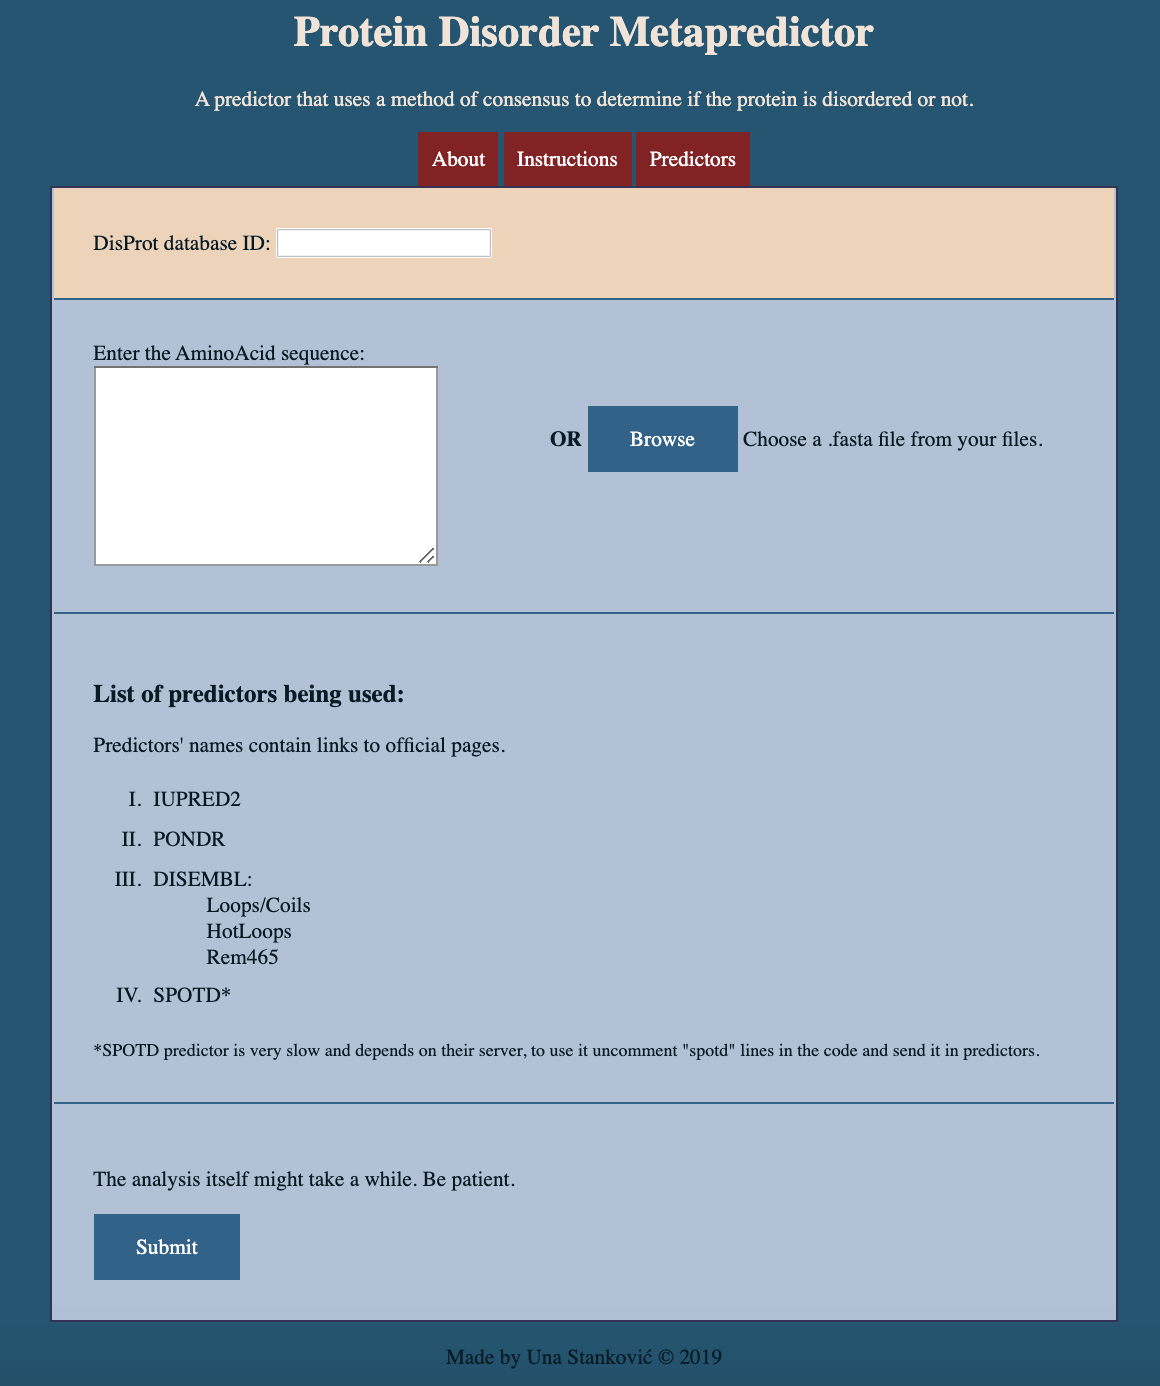
\includegraphics[width=0.7\textwidth]{Figures/App/interfejs.png}
    \caption{Prikaz korisničkog interfejsa}
    \label{fig:interfejs}
\end{figure}

Nakon što server obradi podatke, rezultati se vraćaju klijentu i prikazuju se u vidu nekoliko nizova. Ti nizovi predstavljaju izlaze prediktora, odnosno, njihove odluke o uređenosti (neuređenosti) svake od aminokiselina u sekvenci.\\

U prvom redu predstavljena je sekvenca, aminokiselina po aminokiselina. U ostalim redovima predstavljeni su slovom $"$D$"$ aminokiseline koje pripadaju neuređenim regionima sekvence. Ukoliko je identifikator u $DisProt$ bazi unet, na osnovu njega se očitavaju i prikazuju eksperimentalno neuređeni regioni, koji se nalaze u redu označenom rečju $DisProt$, obeleženi, takođe, slovom $"$D$"$ . \\

U narednom redu se nalazi prosečni skor prediktora (proračunat na osnovu odgovora prediktora, podrazumeva se bez korišćenja informacija iz $DisProt$ baze). Ispod navedenog skora, nalaze se odluke o neuređenosti za sve metaprediktore, kada je bar $k$, $1 \leq k \leq brojprediktora$, prediktora predvidelo neuređenost neke aminokiseline - obeleženo sa $D$. Potom, ukoliko je dat $DisProt$ identifikator, prikazane su vrednosti mera kvaliteta metaprediktora. Ispod kojih se nalazi grafički prikaz prosečne vrednosti skora nad sekvencom i skalom datih rezultata na $y$-osi. \\ 

Na samom kraju, nalazi se tabela koja sadrži podatke o merama kvaliteta metaprediktora u zavisnosti od broja prediktora koji su predvideli da je region neuređen. Posmatra se sledeće tvrđenje: $"$ \textit{Aminokiselina je neuređena ukoliko je $k$ prediktora predvidelo da je neuređena}.$"$Prikaz stranice sa rezultatima može se videti na slici \ref{fig:rezultati}.
\begin{figure}[H]
	\centering
    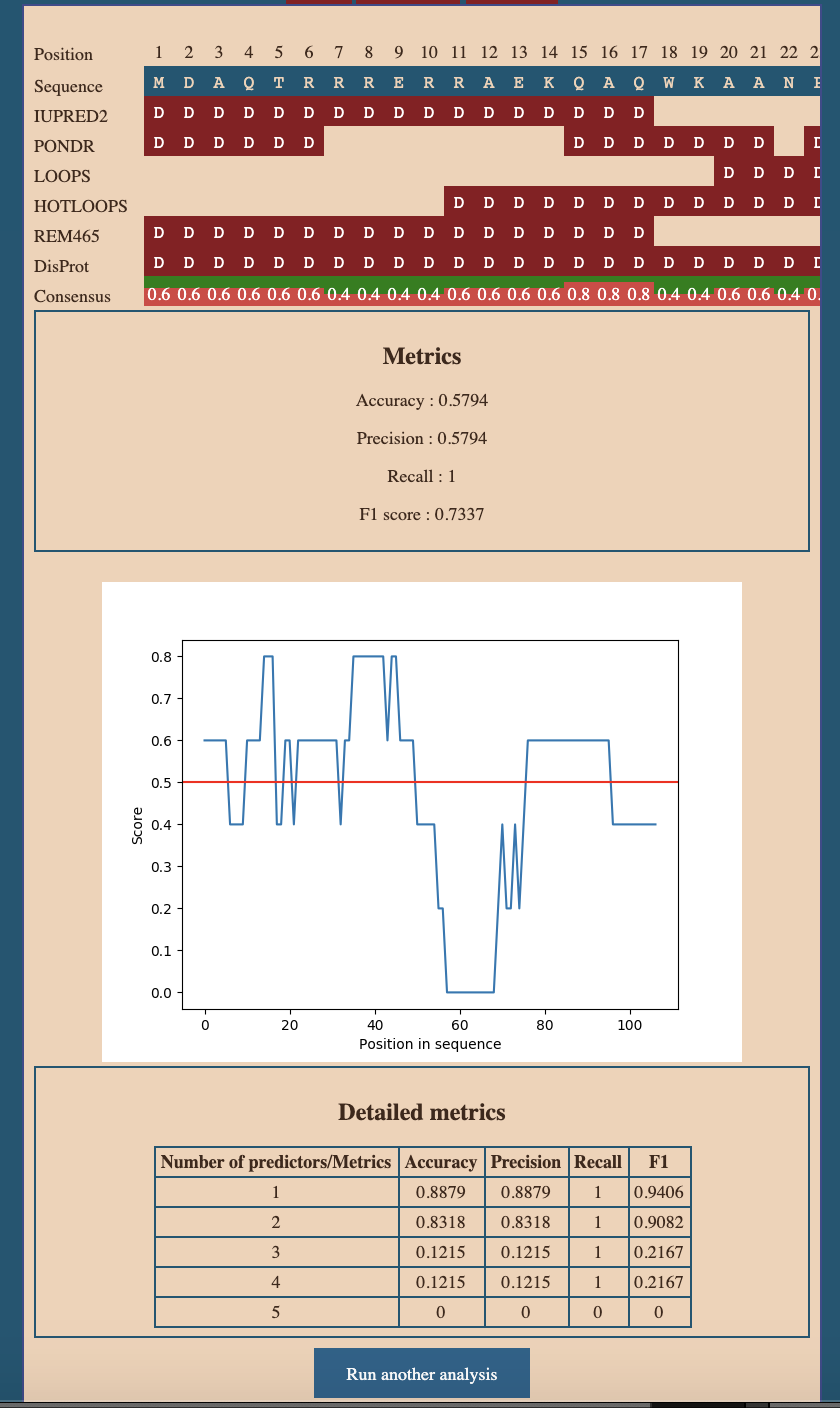
\includegraphics[width=0.7\textwidth]{Figures/App/rezultati.png}
    \caption{Prikaz korisničkog interfejsa pri povratku rezultata sa servera za protein sa identifikatorom $DP00003$}
    \label{fig:rezultati}
\end{figure}

\subsubsection{Implementacija klijenta}
Klijent je implementiran kroz programski jezik JavaScirpt i korišćenjem veb tehnologija $HTML5$ i $CSS3$. 
Ceo kôd klijenta sastoji se iz narednih datoteka:
\begin{itemize}
\item \textbf{index.html} - glavna strana koja od korisnika zahteva unos i sadrži informacije o projektu, uputstvo za korišćenje aplikacije, kao i informacije o prediktorima,
\item \textbf{style.css} - datoteka sadrži sve stilove korišćene kroz aplikaciju,
\item \textbf{sock\_cli.js} - datoteka prikuplja informacije unete od strane klijenta i prosleđuje ih serveru, prima informacije od servera i poziva funkcije iz $results.js$ kako bi se izvršio prikaz dobijenih rezultata na stranici,
\item \textbf{results.js} - datoteka sadrži funkcije za kreiranje prikaza i vrši prikaz dobijenih rezultata na stranici dinamički, kreiranjem novih elemenata, 
\item \textbf{loader.js} - datoteka menja prikaz stranice prilikom čekanja na server.
\end{itemize}

Za komunikaciju sa serverom koristi se $socketio$ biblioteka. Podaci se šalju emitovanjem određenog događaja čiji se naziv navodi kao prvi argument funkcije $emit$. Ukoliko nisu uneti ni sekvenca ni $DisProt$ identifikator, korisnik se obaveštava i zahteva se unos.
\begin{lstlisting}[language=Python]
const socket = io('http://localhost:5000');
socket.on('connect', () => {
    console.log('Connected to server');
});

function sendData() {
    if (txtDisprotId.value == "" && txtSequence.value == ""){
        alert("You must enter the DisProt id or the sequence!");
    }
    else{
        showLoader();
        const json = generateData();
        console.log('Sending to server.');
        socket.emit('message', json);
    }
}
\end{lstlisting}

Primanje podataka vrši se reagovanjem na događaj koji se navodi kao prvi argument funkcije $on$. Kako bi se podaci pravilno prikazali više funkcija za prikaz različitih delova rezultata moraju biti pozvane.\\

\begin{lstlisting}[language=Python]
socket.on('predicted', data => {
    console.log('Got from server.');
    console.log(data);
    hideLoader(); 
    createScale(data.sequence);
    for (const pred of data.predictors) {
        if (pred.result != "")
            createPredictor(pred.result, pred.name);
    }
    createConsensus(data.consensus.result);
    if(data.partial_metrics_cons != ""){
        for (i=1; i < data.num_of_preds+1; i++){
            if(data.partial_metrics_cons[i] != ""){
                const name_pred = "MP " + i;
                createPredictor(data.partial_metrics_cons[i], name_pred);
            }
        }
    }
    if (txtDisprotId.value != ""){ 
        addMetrics(data.metrics);
        addDetailedMetrics(data.partial_metrics);
    }
    else{
        addConsensusImage();
        addReloadButton();
    }
    
});
\end{lstlisting} 

\subsection{Server} 
 Serverska obrada se sastoji iz komunikacije sa lokalno čuvanim aplikacijama (programima za prediktore), kao i postojećim veb stranicama kako bi se obezbedili podaci neophodni za analizu.\\
 
Serverska strana komunicira sa klijentskom stranom korišćenjem soketa, odnosno $socketio$ biblioteke. Ovaj vid komunikacije u kombinaciji sa nitima, je odabran zbog čekanja na izlaze iz prediktora. Ukoliko bi se radilo o nekom drugom vidu komunikacije moglo bi da se desi da se rezultati ne prikažu ili izmešaju zbog neujednačenog vremena povratka informacija. Server slušanjem čeka na informacije od klijenta i po primanju informacija vrši nekoliko radnji:
\begin{itemize}
\item Ukoliko je dostupan \textit{DisProt} \textit{identifikator} šalje se zahtevom preko omogućenog $API$-ja\footnote{API - skraćeno od engl. \em{Application Programming Interface}, predstavlja interfejs za komunikaciju sa, u ovom konkretnom slučaju, $DisProt$ $bazom$. }. Odgovor se, potom, parsira regularnim izrazima kako bi se dobili eksperimentalno neuređeni regioni - intervali regiona u sekvenci i sekvenca. Potom se ti intervali popunjavaju u listi i koja se vraća kao niz karaktera $"$D$"$ i $"$-$"$, gde $"$D$"$ predstavlja neuređenost.
\item Sekvenca se smešta u zasebnu datoteku, za potrebe lokalno čuvanih prediktora. Osim toga, sekvenca se dodatno parsira (ukoliko je zadata u $.fasta$ formatu iz nje se uklanja prva linija, kako bi bila prilagodjena za ulaz prediktorima koji zahtevaju samo sirovu sekvencu).
\item Sekvenca se šalje prediktorima. Prediktori su kreirani kao elementi klase $Predictor$ i za svaki od njih se računa $calculate$ funkcija koja vraća listu karaktera $"$D$"$ i $"$-$"$.
\item Svaki od prediktora prima sekvencu i na poseban način je obrađuje:
	\begin{itemize}
	\item \textit{IUPRED2} - Prediktor se nalazi lokalno sačuvan i prosleđuje mu se naredba za pokretanje, kao i naziv datoteke u kojoj je sačuvana niska koja se obrađuje.  
	\item \textit{PONDR} - Prediktor se nalazi na $veb$  \href{http://www.pondr.com/cgi-bin/pondr.cgi}{lokaciji} na kojoj se nalazi forma koja se dinamički popunjava na osnovu korisničkog unosa uz pomoć $mechanize$ modula. Potom se regularnim izrazom parsira dobijeni rezultat.  
	\item \textit{SPOTD} - Prediktor se nalazi na $veb$ \href{http://sparks-lab.org/server/SPOT-disorder/}{lokaciji} i postupak je poput prethodnog prediktora, međutim, problem koji se javlja sa ovim prediktorom je taj što je server poprilično spor (izvršavanje preko 10 minuta, server često nije dostupan). Za korišćenje ovog prediktora neophodno je skinuti komentare iz koda i dodati u $predictors$ objekat rezultat $spotd$ predikcije.
	\item \textit{DISEMBL} - Prediktor predstavlja spoj tri prediktora $coils/hotcoils$, $loops$ i $rem465$ . Prediktor se nalazi na $veb$ \href{http://dis.embl.de/cgiDict.py}{lokaciji}. Ovaj prediktor vraća rezultate na osnovu tri vida predikcije. 
	\end{itemize}
\end{itemize}

\subsubsection{Implementacija servera}
Serverska strana je u potpunosti implementirana u programskom jeziku $Python$ i organizovana je kroz sledeće datoteke:
\begin{itemize}
\item \textbf{sock\_serv.py} - Datoteka sadrži srž serverske strane programa. U datoteci su organizovani primanje informacija sa servera i emitovanje povratnih informacija. 
\item \textbf{predictor\_service.py} - Datoteka sadrži kreiranje elemenata klasa i vraća izračunate vrednosti predikcije.  
\item \textbf{disprot\_service.py} -U ovoj datoteci se nalazi povezivanje na   \textit{DisProt} bazu i parsiranje dobijenih rezultata. Iz dobijenih informacija iz baze zanimaju nas intervali koji sadrže neuređene regione i sekvenca. Iako su pored regiona obezbeđene informacije o metodu kojim su oni određeni, za ovaj rad ti podaci nisu relevantni. 
\item \textbf{predictor.py} - Datoteka sadrži kreiranu klasu \textit{Predictor}, i metode koje su neophodne za svaki od prediktora.  
\item \textbf{consensus.py} - Datoteka sadrži funkcije vezane za kreiranje konsenzusa i iscrtavanje rezultata.
\item \textbf{measures.py} - Datoteka sadrži funkcije vezane za formiranje mera kvaliteta metaprediktora. 
\item \textbf{pondr.py}  
\item  \textbf{spotd.py}  
\item \textbf{iupred2.py}  
\item \textbf{disembl.py}  
\end{itemize}
Poslednje navedene datoteke sadrže informacije opisane u prethodnoj podeli, svaki rezultat je predstavljen u vidu liste. 

Za komunikaciju sa klijentom, koristi se $socketio$ biblioteka, koja funkcioniše po istom principu kao na klijentskoj strani. Konekcija sa klijentom je realizovana na sledeći način:

\begin{lstlisting}[language=Python]
sio = socketio.Server(cors_allowed_origins=['http://localhost:9004'])
app = socketio.WSGIApp(sio, static_files={
    '/': {'content_type': 'text/html', 'filename': 'index.html'}
})

@sio.event
def connect(sid, environ):
    print('connect ', sid)
    
if __name__ == '__main__':
    eventlet.wsgi.server(eventlet.listen(('', 5000)), app)
\end{lstlisting}

Primanje informacija od klijenta funkcioniše tako što server sluša čekajući na poruku i po prijemu poruke poziva funkciju za pozivanje prediktora.
\begin{lstlisting}[language=Python]
@sio.on("message")
def message(sid, data):
    print('message ', data)
    
    # Calling all the predictors to give their opinion on the sequence in the same thread!
    x = threading.Thread(target=prediction_calls(data), args=(data))
    x.start()
\end{lstlisting}

Funkcija za pozivanje prediktora se sastoji iz nekoliko celina:
\begin{enumerate}
\item Najpre se iz prosleđenih podataka izvlače informacije o $prediktorima$, $identifikatoru$ i $sekvenci$ (u zavisnosti od toga šta je zadao korisnik). 
\begin{lstlisting}[language=Python]
def prediction_calls(data):
    id_disp = data["disprot_id"]
    s = data["sequence"]
    # DisProt database call
    [disprot, seq] = disprot_service.get_sequence_info(id_disp)
    print(seq, len(seq))
    if (s == ""):
        s = seq
	predictors_all = []
	predictors_object = []
    
	for i in range(0, len(data["predictors"])):
        p = data["predictors"][i]
        pred = {}
        pred["name"] = p.upper()
        if p == "iupred2":
            pred["result"] = iupred2
            predictors_all.append(iupred2) 
        if p == "pondr":
            pred["result"] = pondr
            predictors_all.append(pondr)   
        if p == "loops":
            pred["result"] = loops
            predictors_all.append(loops)
        if p == "hotloops":
            pred["result"] = hotloops
            predictors_all.append(hotloops)  
        if p == 'rem465':
            pred["result"] = rem465
            predictors_all.append(rem465)
        predictors_object.append(pred)
\end{lstlisting}
Identifikator se prosleđuje $get\_sequence\_info$ u datoteci $disprot\_service.py$ koja dohvata informacije iz baze. Pripremanje sekvence sastoji se iz parsiranja povratnih informacija sa servera, izvlačenja intervala i popunjavanja pozicija tih intervala sa $"$D$"$.
\begin{lstlisting}[language=Python]
def get_sequence_info(id_disp):
   # response = requests.get('http://www.disprot.org/ws/get/' + id_disp) # Old API changed on 13.09.2019.
    response = requests.get('http://www.disprot.org/api/' + id_disp)
    data = json.loads(response.content)
    if re.search("200", str(response)) == None:
        data = "Not found."
    return prepare_sequence(data)
    
def prepare_sequence(data):
    if data == "Not found.":
        return data
    sequence = data['sequence']
    seq_len = len(shortened_sequence(sequence)) 
    intervals = []
    disprot = []
    disprot = ['-'] * seq_len
    for record in data['regions']:
        start_interval = record["start"]
        end_interval = record["end"]
        intervals.append((start_interval, end_interval))
    for interval in intervals:
        begin, end = int(interval[0]), int(interval[1])
        for i in range(begin-1, end):
            disprot[i] = "D"
    return disprot, sequence
\end{lstlisting}

\item Potom se sekvenca (bez obzira na to da li je iz $DisProt$ baze ili je zadata drugačije) čuva lokalno u fajlu. Ovo je neophodno kako bi mogla da bude ulaz za lokalno dostupni prediktor $IUPRED$.
\begin{lstlisting}[language=Python]
 # Storing the sequence in a file in order to locally use the predictors
    f = open("sequence.txt", "w")
    f.write(s)
    f.close()
\end{lstlisting}
\item Nakon toga pozivaju se prediktori da pojedinačno daju rezultat. Prediktor $SPOTD$ je izuzet iz računanja, jer zavisi od njihovog servera koji je često nedostupan ili veoma spor	. 
\begin{lstlisting}[language=Python]
# Calling predictors
    iupred2 = predictor_service.iupred2_predict(s)
    #SPOTD: uncomment the function call 
    #spotd = predictor_service.spotd_predict(s) 
    pondr = predictor_service.pondr_predict(s)
    ss = shortened_sequence(s)
    [loops, hotloops, rem465] = predictor_service.disembl_predict(ss)
\end{lstlisting}
Prilikom poziva prediktora, unutar funkcija oblika $nazivprediktora\_predict$, kreira se instanca klase $Predictor$ za datu sekvencu, a vraća se izračunat rezultat predikcije kroz polje $self.calculated$. Navedene funkcije nalaze se u datoteci $predictor\_service.py$. Metod $calculate()$ za svaku instancu klase $Predictor$ izračunava neuređene regione i smešta ih u $self.calculated$.
\begin{lstlisting}[language=Python]
def iupred2_predict(sequence):
    p = iupred2(sequence)
    return p.calculate()

def spotd_predict(sequence):
    p = spotd(sequence)
    return p.calculate()

def pondr_predict(sequence):
    p = pondr(sequence)
    return p.calculate()

def disembl_predict(sequence):
    p = disembl(sequence)
    return p.calculate() 
\end{lstlisting}
Izgled klase $Predictor$ iz datoteke $predictor.py$.
\begin{lstlisting}[language=Python]
class Predictor:
    def __init__(self, sequence):
        self.sequence = sequence
        self.calculated = []

    def calculate(self):
        pass # Store result in self.calculated in form [aa1_prediction, aa2_prediction, aa3_prediction, ...]
\end{lstlisting}
Za prediktore kojima se pristupa preko njihovih veb stranica koristi se biblioteka $mechanize$ za popunjavanje odgovarajućih formi i biblioteka $re$ kojom se uvode regularni izrazi, neophodni za parsiranje dobijenih rezultata. Primer izgleda jednog od prediktora kod koga se predikcija vrši preko veb stranice:
\begin{lstlisting}[language=Python]
class pondr(Predictor):
    def calculate(self):
      global br
      url = "http://www.pondr.com/cgi-bin/pondr.cgi" 
      br.set_handle_robots(False)
      br.open(url)
      br.form = list(br.forms())[1] 
      br['ProteinName'] = "test"
      br['Sequence'] = self.sequence 
      response = br.submit()
      soup = BeautifulSoup(response.read(), features='html5lib')
      soup = soup.prettify()
      result = re.findall("VLXT\t\s.*", soup)
      # We don't need the first one because it is not sequence
      result = result[1:]
      predicted = []
      for r in result:
          pred = r[6:]
          predicted.append(pred)
      total = []
      # Getting everything in one sequence 
      for i in predicted:
        total += i
      old = len(total)
      
      pom = shortened_sequence(self.sequence)
      if(old < len(self.sequence)):
        for i in range(0,len(pom) - old):
          total.append(" ")
      total = [x if x != ' ' else '-' for x in total ]
      
      self.calculated = total
      return self.calculated
\end{lstlisting}
\item Računa se prosečna vrednost skora predikotra, a potom se računaju procene mera kvaliteta prediktora uz pomoć funkcije $measure\_all$ koja se nalazi u datoteci $measure.py$.  Prvo se ovaj postupak radi za ceo metaprediktor, a potom za svaki koji koristi $k$ prediktora pojedinačno. U slučaju da $DisProt$ identifikator nije unet, neophodno je vratiti prazne niske za rezultate.
\begin{lstlisting}[language=Python]
    cons = consensus(ss, predictors_all)
    cons_decs = {}
    for i in range(1,len(predictors_all)+1):
        cons_tres = consensus_treshold(cons,1/len(predictors_all)*i)
        cons_decs[i] = cons_tres
    if (id_disp != ""):
        bin_disprot = binarize_values(disprot)
        m = measure_all(consensus_treshold(cons), bin_disprot)
        # Doing consensus and metrics for when one, two or more predictors said "D"
        consensus_values = {}
        for i in range(1,len(predictors_all)+1):
            consensus_values[i] = measure_all(cons_tres, bin_disprot) 
        pred = {}
        pred['name'] = "DisProt"
        pred['result'] = disprot
        predictors_object.append(pred) 
        print(predictors_object)
    else:
        # If there is no DisProt id, only predictors results should be displayed.
        m = []
        for i in range(0,4):
            m.append("")
        consensus_values = ""
        disprot = ""   

\end{lstlisting}
Za računanje prosečne vrednosti skora prediktora koristi se funkcija $consensus$ iz datoteke $consensus.py$, koja prima dva argumenta: sekvencu i listu rezultata prediktora. Ona za svaku od pozicija u rezultatu prediktora i za svaki od prediktora, posmatra da li je aminokiselina neuređena na toj poziciji i, ako jeste, dodaje jedinicu na ukupan skor za tu poziciju. Da bi se dobio konsenzus, nakon što su svi prediktori dali odluku o nekoj poziciji akumulirana vrednost u $val$ se deli sa brojem prediktora. Na kraju se poziva funkcija za iscrtavanje grafika konsenzusa.
\begin{lstlisting}[language=Python]
def consensus(sequence, predictors):
    num_of_preds = len(predictors)
    score = []
    for i in range(0, len(sequence)):
        val = 0
        for pred in predictors:
            if pred[i] == 'D':
                val += 1
        score.insert(i, val / num_of_preds)
    plot_consensus(score, sequence)
    return score
\end{lstlisting}
Kako bi se odredili prosečna vrednost skora i mere kvaliteta metaprediktora kada treba da se posmatra slučaj da je jedan, dva ili više prediktora predvidelo da je region neuređen, vrši se nekoliko poziva:
\begin{itemize}
\item funkcija $consensus\_treshold$ iz datoteke $consensus.py$, vraća binarizovani konsenzus u odnosu na neki prag (eng. \em{treshold}). Prag se računa tako što se broj prediktora koje želimo da uračunamo deli sa ukupnim brojem prediktora. 
\begin{lstlisting}[language=Python]
def consensus_treshold(cons, treshold=0.5):
    new = []
    print(treshold)
    for c in cons:
        if c >= treshold:
            new.append(1)
        else:
            new.append(0)
    return new
\end{lstlisting}
\item funkcija $measure\_all$ prima dva argumenta binarizovani niz konsenzusa i binarizovani niz vrednosti iz $DisProt$ baze. Binarizaciju je neophodno izvršiti kako bi ulazi bili pogodni za algoritme za računanje mera kvaliteta, ona se vrši funkcijom $binarize\_values$ iz datoteke $measures.py$.
\begin{lstlisting}[language=Python]
def measure_all(x,y):
    a = round(m.accuracy_score(x, y), 2)
    p = round(m.precision_score(x, y), 2)
    f = round(m.f1_score(x, y), 2)
    r = round(m.recall_score(x, y), 2)
    return [a, p, r, f]
    
def binarize_values(x):
    new = []
    for el in x:
        if el == "D":
            new.append(1)
        else:
            new.append(0)
    return new
\end{lstlisting}
\end{itemize}

\item Na kraju se dobijeni rezultati pakuju u objekat koji se potom emituje.

\begin{lstlisting}[language=Python]
result = {
                "predictors": predictors_object,
                "consensus": {
                    'name': 'cons',
                    'result': cons
                },
                "sequence": ss,
                "metrics" : [
                    {
                        'name': 'Accuracy',
                        'result' : m[0]
                    },
                    {
                        'name': 'Precision',
                        'result': m[1] 
                    },
                    {
                        'name': 'Recall',
                        'result': m[2] 
                    },
                    {
                        'name': 'F1 score',
                        'result': m[3] 
                    }
                ],
                "partial_metrics": consensus_values,
                "partial_metrics_cons": cons_decs,
                "num_of_preds": predictors_num
            }
            
    sio.emit('predicted', result)
\end{lstlisting}
\end{enumerate}
% -------------------------------------------------------------------------------------------------

\section{Korišćenje aplikacije}
% -------------------------------------------------------------------------------------------------
Korišćenje aplikacije je veoma jednostavno i linearno. Od korisnika se očekuje da obezbedi $DisProt$ identifikator i/ sekvencu ($.fasta$ datoteke). Postoji tri načina unosa podataka:
\begin{itemize}
\item Prvi način je odabirom proteina iz $DisProt$ baze i unošenjem njegovog identifikatora. Ovaj način ne zahteva i unos sekvence, jer se ona može uzeti iz baze.
\item Drugi način je davanjem samo $DisProt$ identifikatora, a potom preuzimanjem $.fasta$ datoteka iz $UniProt$ baze. Za svaki unos u $DisProt$ bazi, postoji veza ka unosu u $UniProt$ bazi. 
\item Treći način je unosom samo sekvence, bez davanja $DisProt$ identifikatora. Ovim način se razlikuje od prethodna dva, zbog toga što se ne dobijaju mere procene kvaliteta.
\end{itemize} 
Korišćenje aplikacije se svodi na naredni skup koraka:
\begin{enumerate}
\item Unos $DisProt$ $identifikator$ i/ili sekvencu. Ukoliko se sekvenca unosi iz datoteke, onda se klikom na $Browse$ dugme vrši odabir datoteke.
\item Klik na $Submit$ dugme.
\item Pregled rezultata.
\end{enumerate}

\subsection{Primer upotrebe}
% -------------------------------------------------------------------------------------------------
\subsubsection{Prvi primer - zadavanje DisProt identifikatora}
Za prvi primer upotrebe biće uzeta niska sa identifikatorom $DP00003$ u $DisProt$ bazi. 
Niska je odabrana iz $DisProt$ baze, kao što se može videti na slici \ref{fig:DisProt}. Odgovarajuća $.fasta$ datoteka je dostupna u $Uniprot$ bazi podataka. Prikaz dela veb stranice navedene baze i identifikatora niske nalazi se na slici \ref{fig:UniProt}. Za prvi primer upotrebe odabran je unos samo $DIsProt$ identifikatora.

\begin{figure}[H]
	\centering
    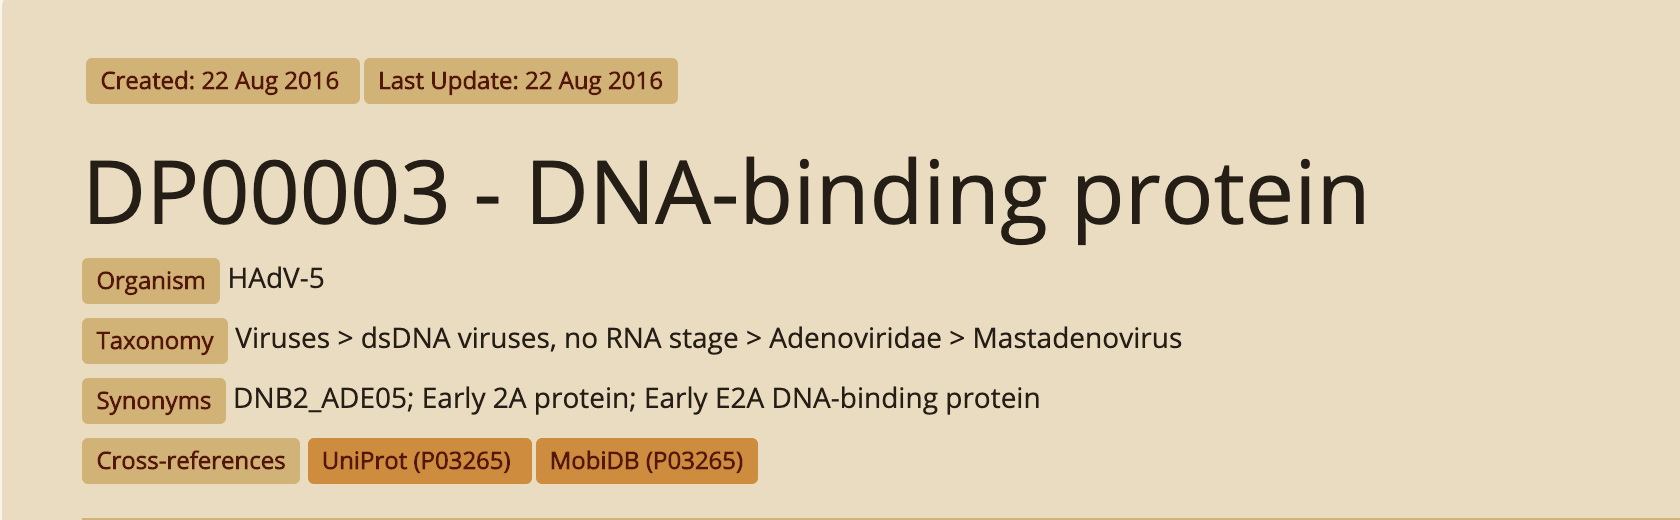
\includegraphics[width=0.7\textwidth]{Figures/App/DisProt.png}
    \caption{Prikaz $DisProt$ baze}
    \label{fig:DisProt}
\end{figure}

\begin{figure}[H]
	\centering
    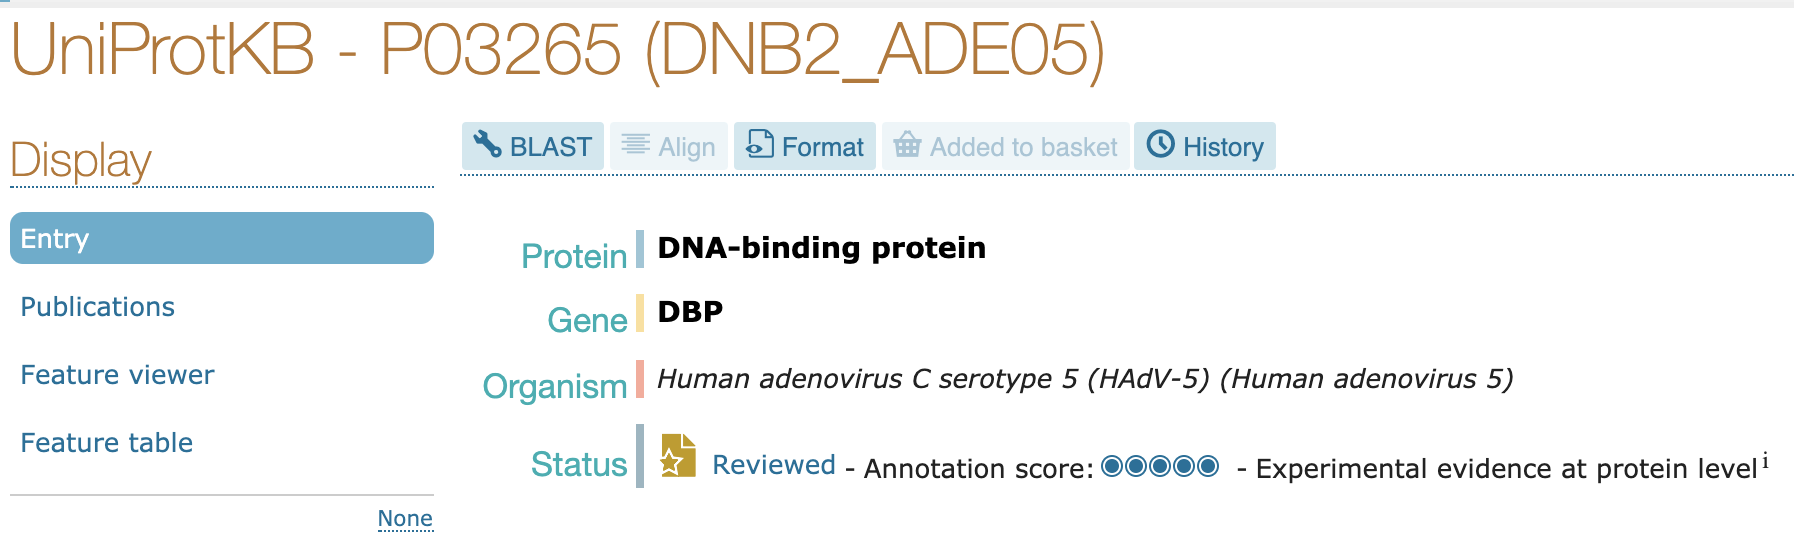
\includegraphics[width=0.7\textwidth]{Figures/App/UniProt.png}
    \caption{Prikaz $UniProt$ baze}
    \label{fig:UniProt}
\end{figure}

Aplikacija nudi korisniku mogućnost da unese identifikator ili sekvencu proteina u odgovarajuća polja za unos teksta što je prikazano na slici  \ref{fig:poljaunos}.

\begin{figure}[H]
	\centering
    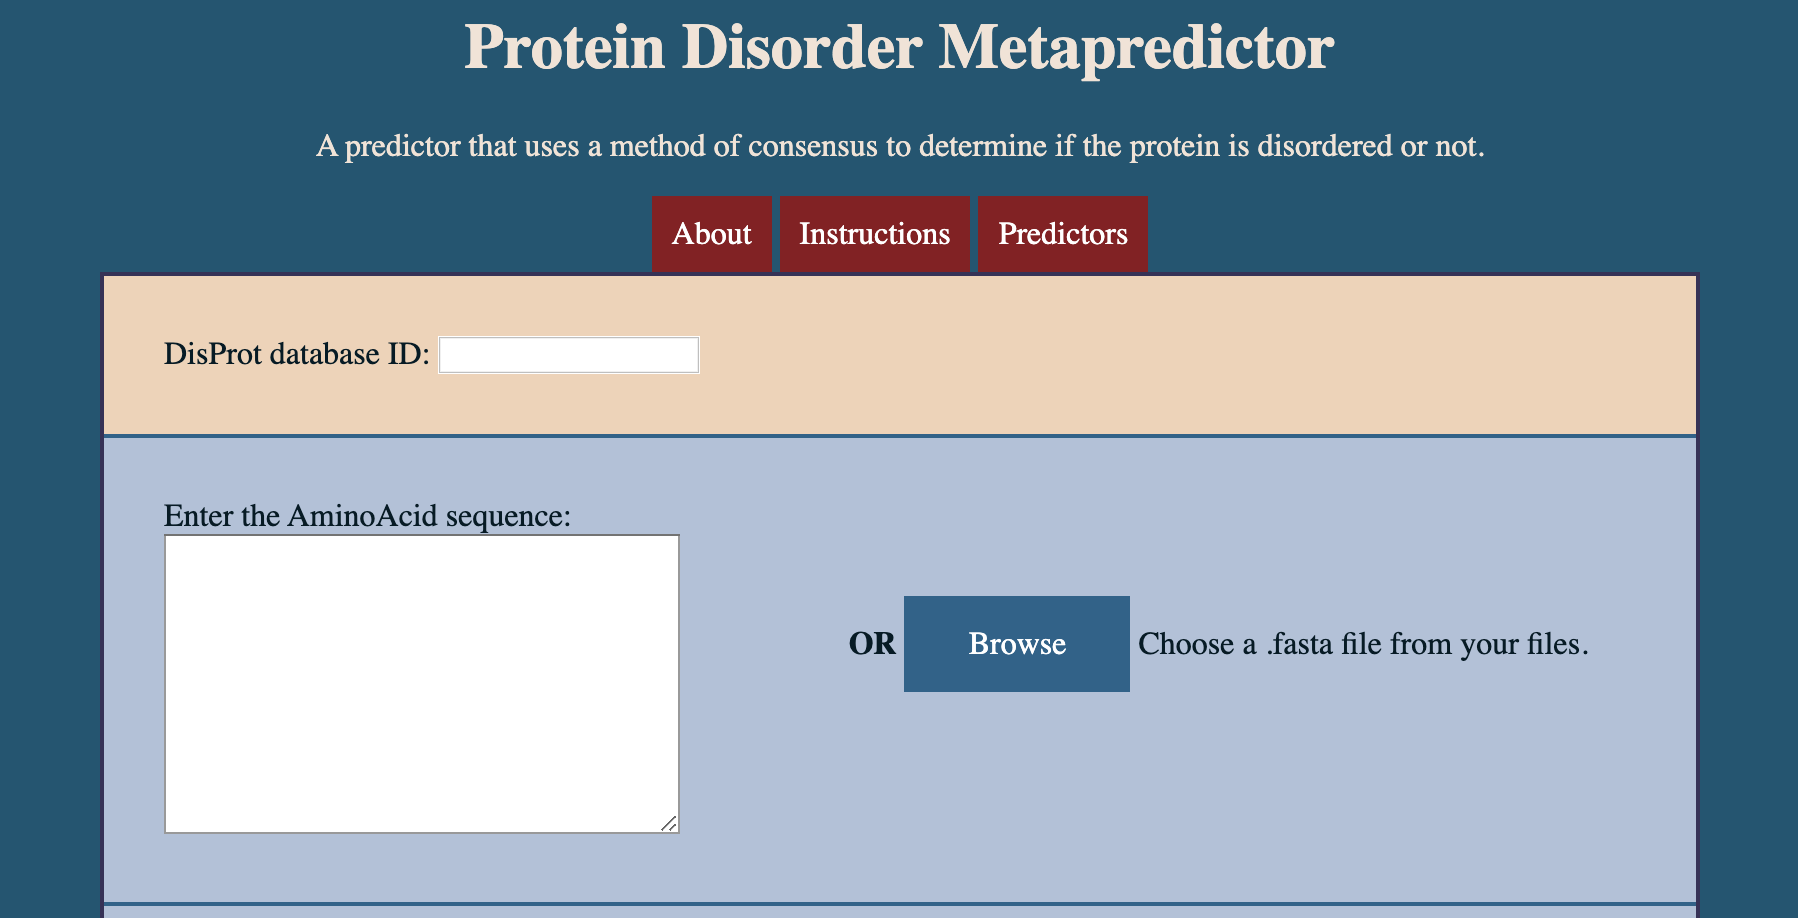
\includegraphics[width=0.7\textwidth]{Figures/App/first_screen.png}
    \caption{Prikaz polja za unos}
    \label{fig:poljaunos}
\end{figure}
Nakon zadavanja ulaznih podataka, proteinska sekvenca se prikazuje u tekstualnom polju čime se dobija izgled kao na slici \ref{fig:unos}.
\begin{figure}[H]
	\centering
    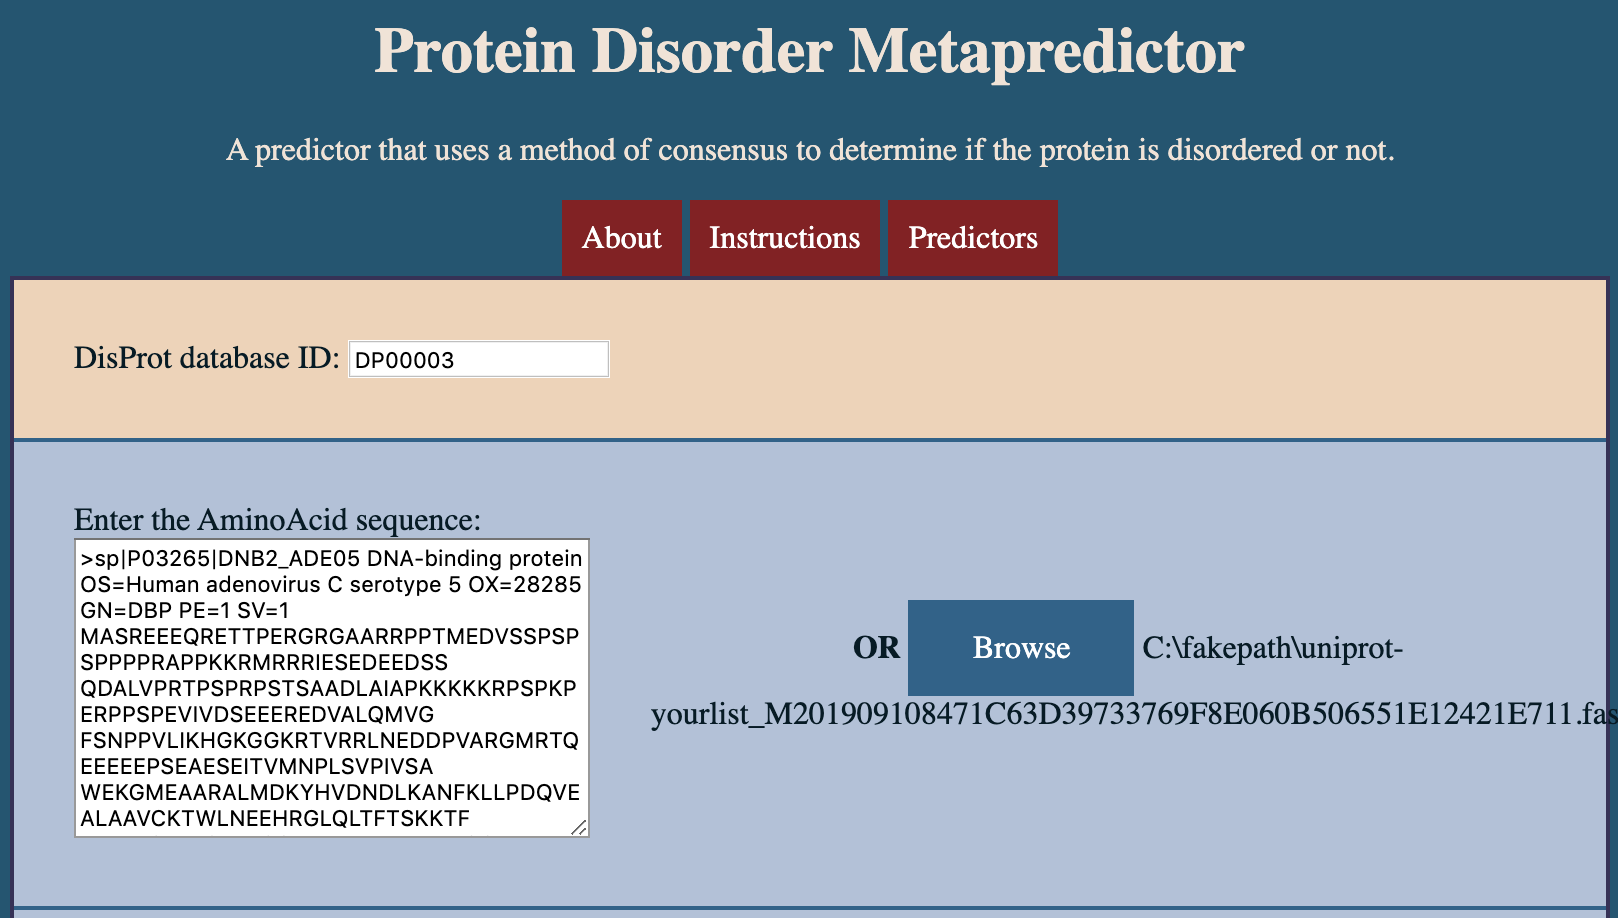
\includegraphics[width=0.7\textwidth]{Figures/App/second_screen.png}
    \caption{Prikaz polja za unos nakon popunjavanja}
    \label{fig:unos}
\end{figure}
Nakon toga, kretanjem ka dnu strane (prikazano na slici \ref{fig:browse}) nailazi se na spisak dostupnih prediktora, gde je moguće izvršiti odabir prediktora, kao i veze ka njihovim zvaničnim stranicama. Klikom na dugme $"$Submit$"$ podaci se šalju na server. U ovom primeru, nije odabran nijedan prediktor, odnosno, odabrani su svi prediktori. 
\begin{figure}[H]
	\centering
    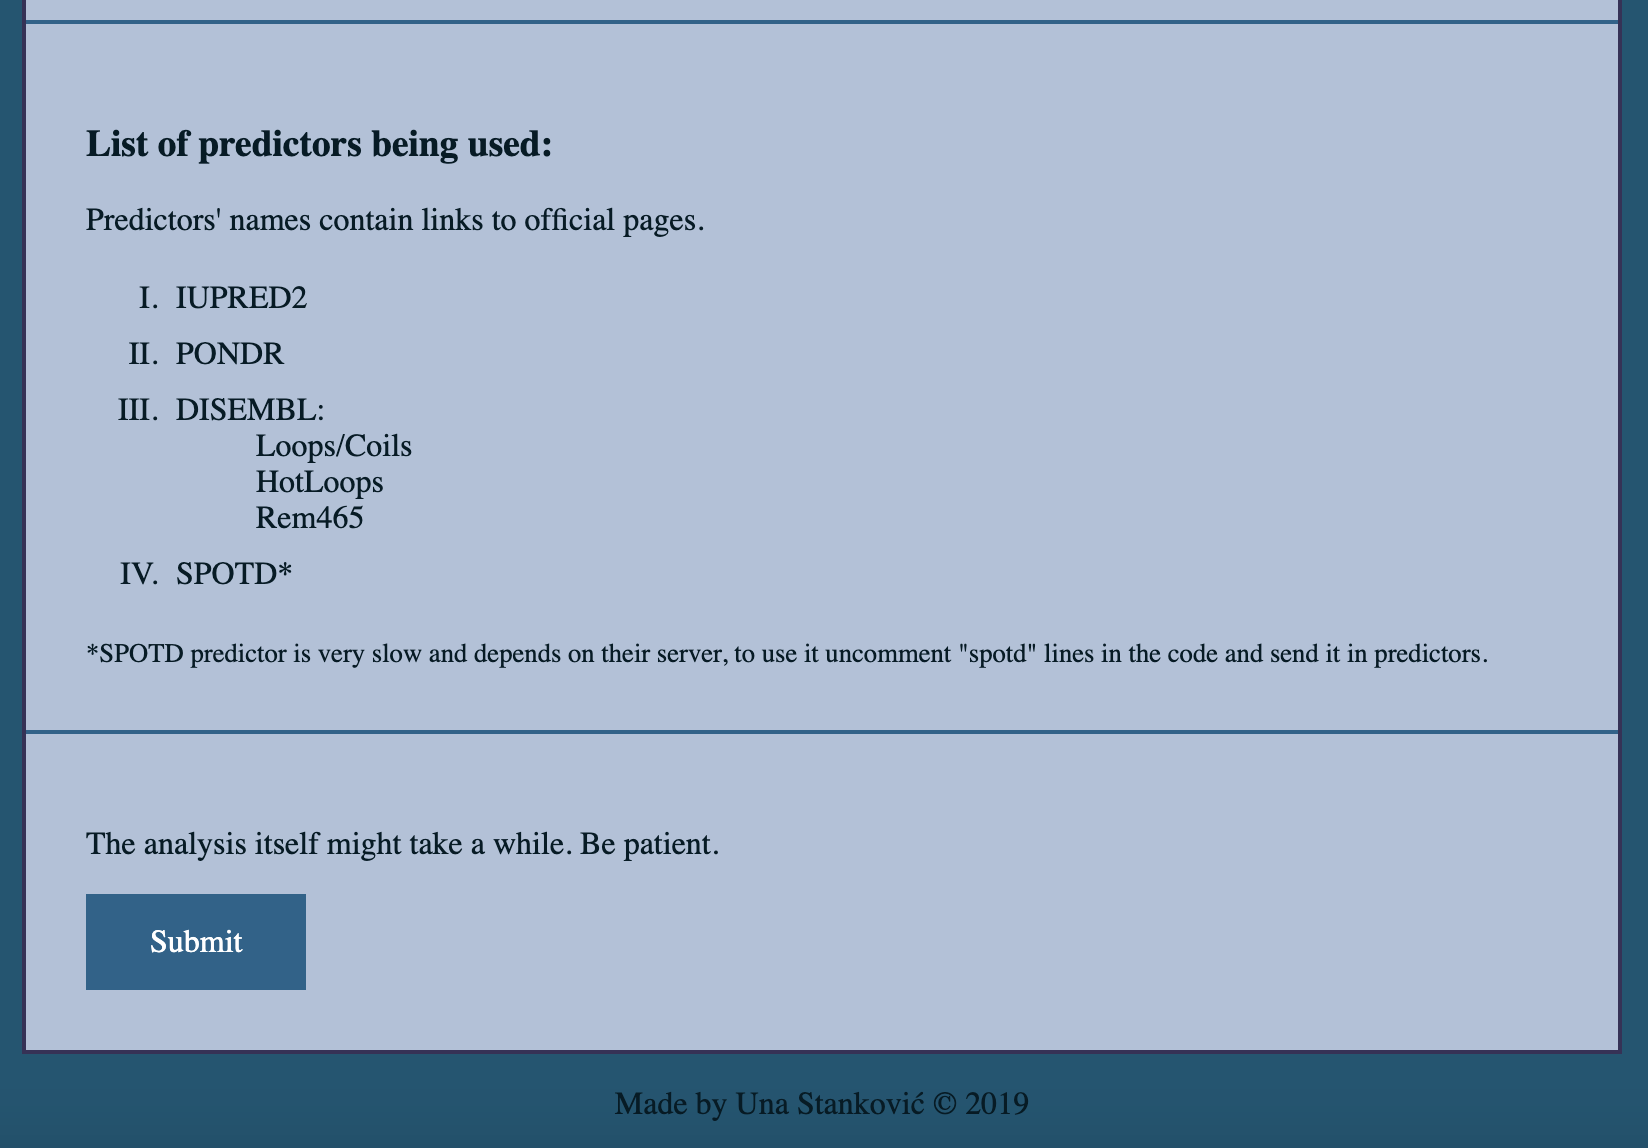
\includegraphics[width=0.7\textwidth]{Figures/App/third_screen.png}
    \caption{Prikaz liste dostupnih prediktora i slanja informacija ka serveru}
    \label{fig:browse}
\end{figure}
Potrebno je neko vreme da se sva izračunavanja izvrše, a potom se pojavljuje strana sa rezultatima. Sa leve strane navedeni su prediktori koji su učestvovali u davanju odluka, neuređeni regioni iz $DisProt$ baze (ukoliko je zadat identifikator), kao i prosečnu vrednost skorova za svaku aminokiselinu po svim prediktorima, pri čemu se podrazumeva da prediktor dodeljuje određenoj aminokiselini skor 1 ako je predvideo da je neuređena, a 0 u suprotnom.	 Procentualno, shodno visini prosečne vrednosti skorova, polje je obojeno u crveno. Ispod skorova, nalazi se prikaz neuređenih aminokiselina za metaprediktor koji koristi $k$ prediktora. Prikaz stranice sa opisanim rezultatima nalazi se na slici \ref{fig:results}.
\begin{figure}[H]
	\centering
    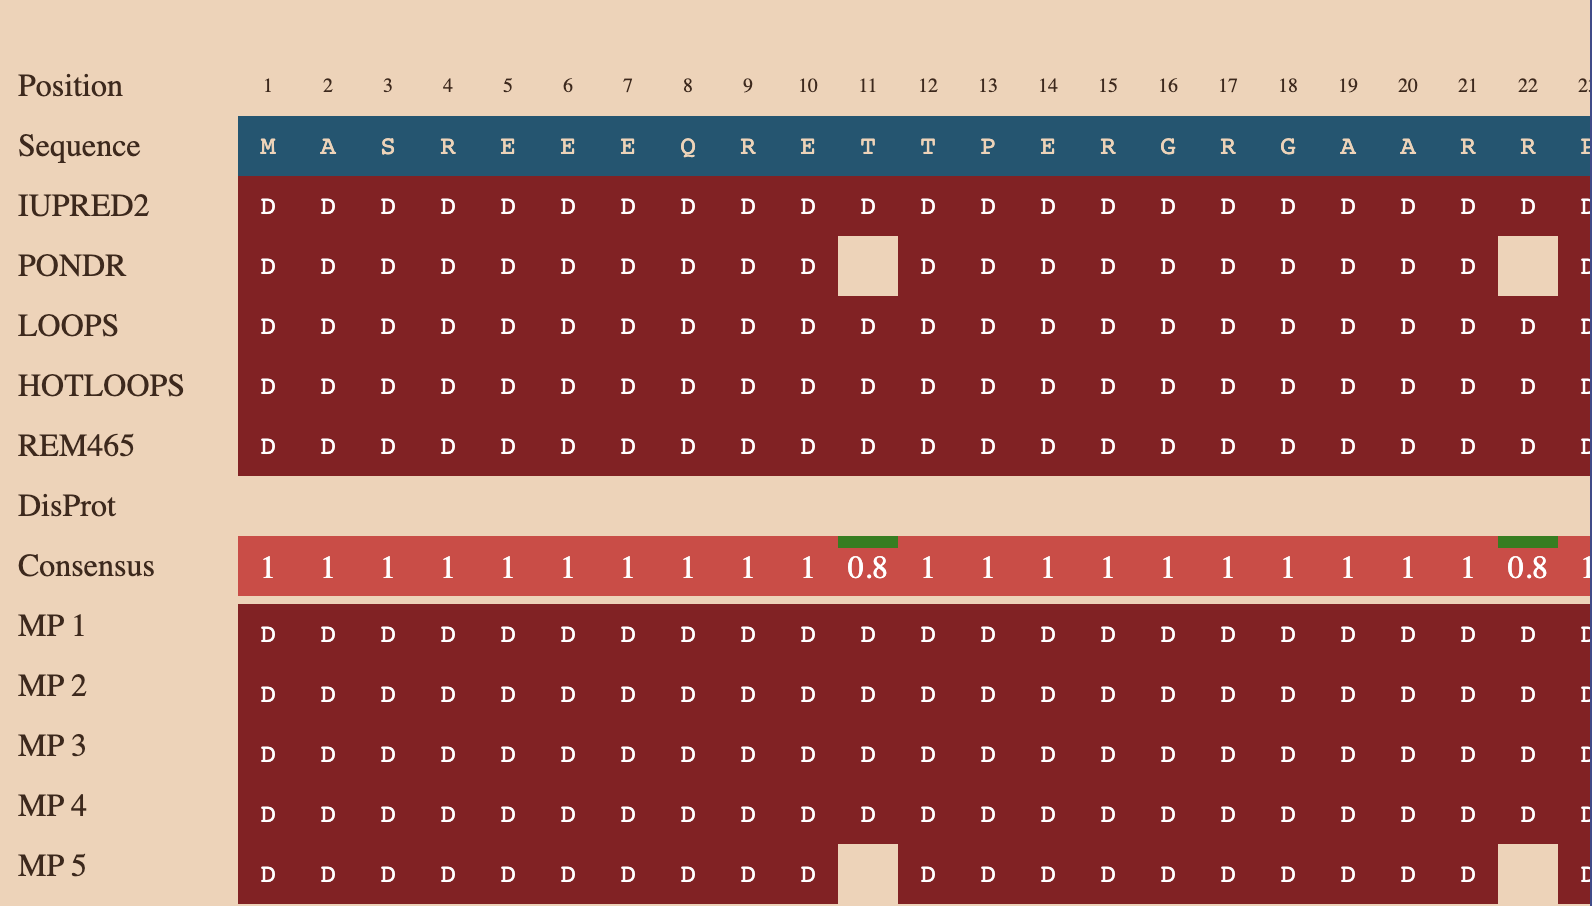
\includegraphics[width=0.7\textwidth]{Figures/App/fourth_screen.png}
    \caption{Prikaz dobijenih rezultata}
    \label{fig:results}
\end{figure}
Uzimajući u obzir da je dužina sekvenci koja se posmatra obimna i da je nemoguće izvršiti prikaz u okvirima stranice, omogućen je pregled cele sekvence, pomeranjem na levo sa dužinom sekvence kao što se može videti na slici \ref{fig:disprotrez}.
\begin{figure}[H]
	\centering
    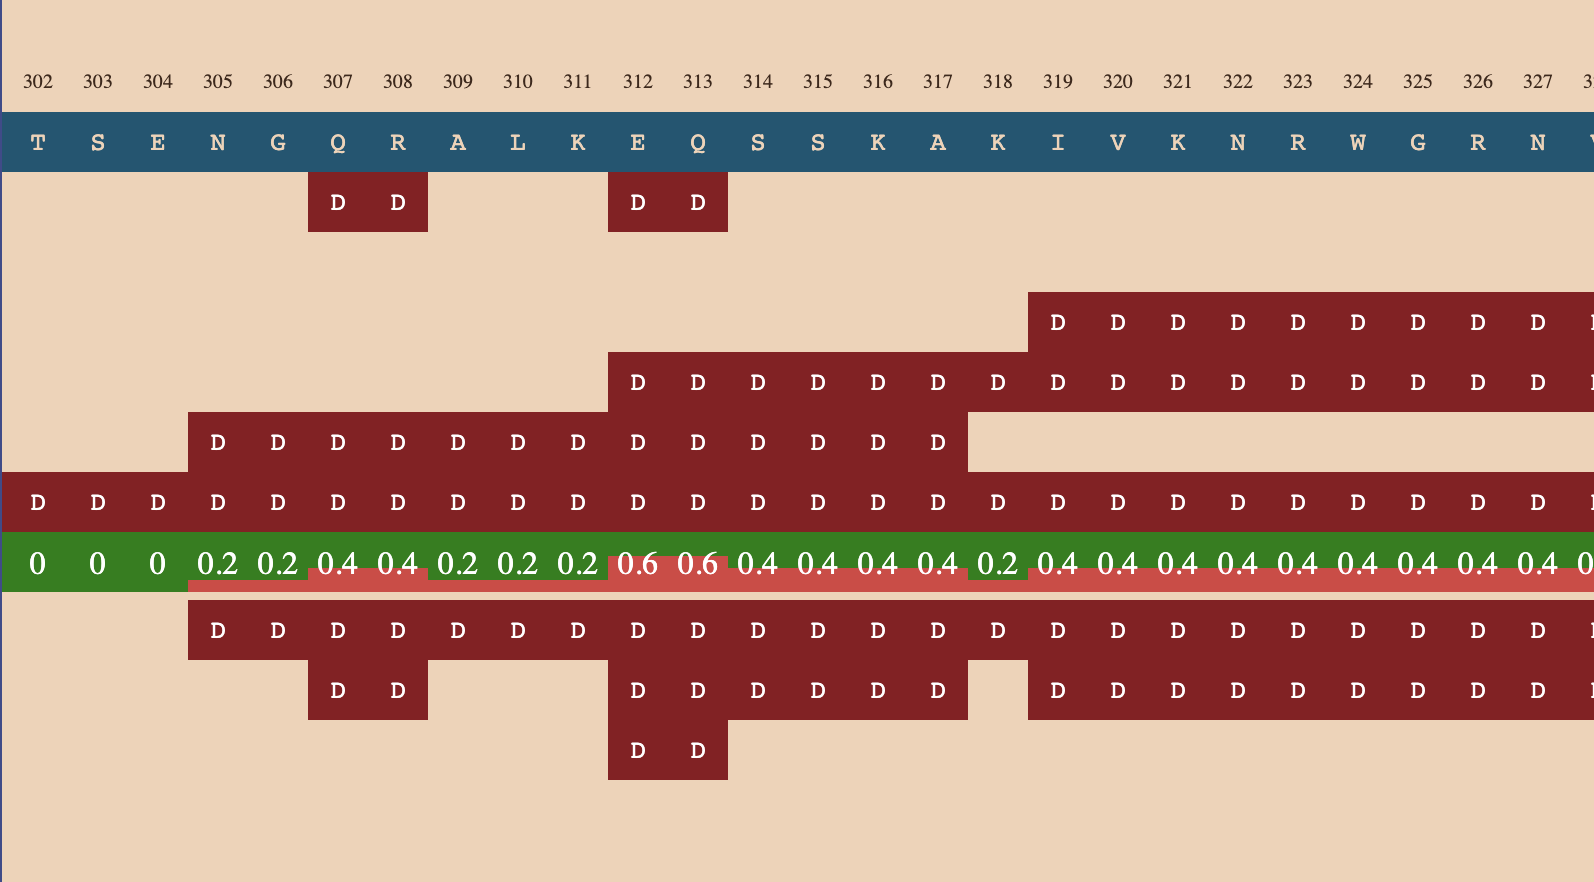
\includegraphics[width=0.7\textwidth]{Figures/App/fifth_screen.png}
    \caption{Prikaz dobijenih rezultata na kom se vidi i izlaz iz $DisProt$ baze}
    \label{fig:disprotrez}
\end{figure}

Ispod navedenih rezultata, ukoliko je dat $DisProt$ identifikator, nalazi se prikaz vrednosti mera kvaliteta metaprediktora za datu prosečnu vrednost skora i rezultate iz $DisProt$ baze. U obzir su uzete četiri statističke mere: tačnost, preciznost, odziv i F1 mera. Izgled prikaza procenjenih mera vidi se na slici \ref{fig:grafik}

\begin{figure}[H]
	\centering
    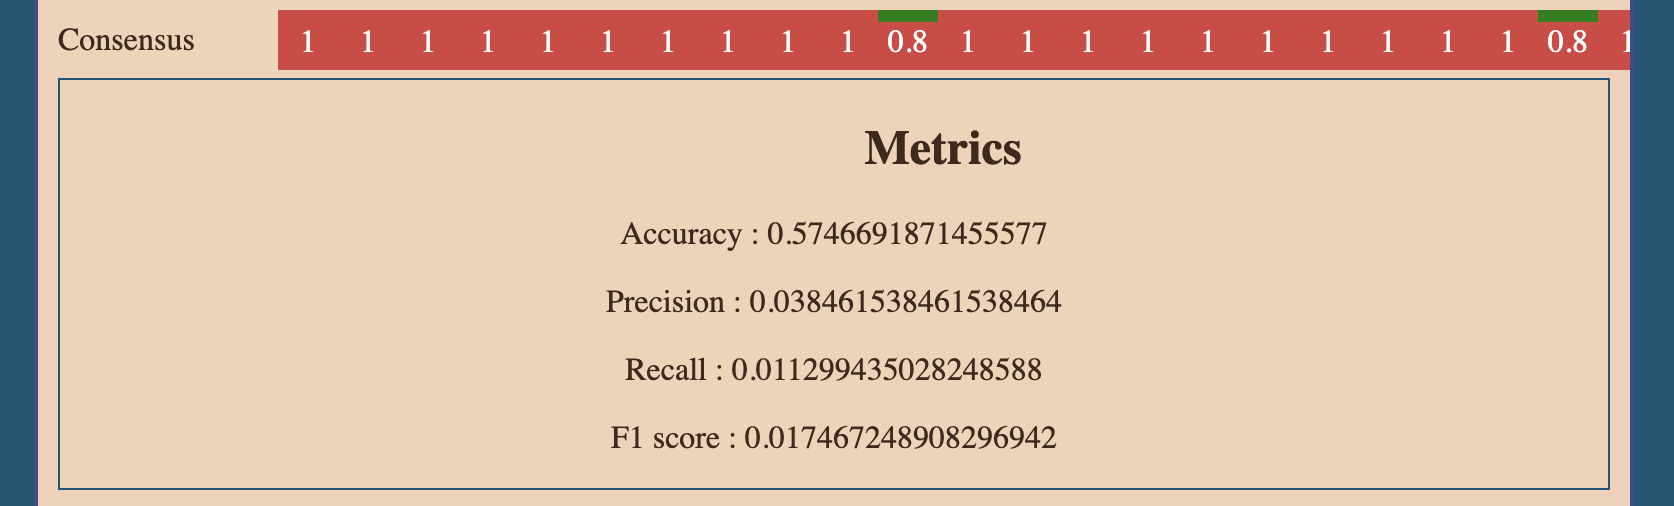
\includegraphics[width=0.7\textwidth]{Figures/App/seventh_screen.png}
    \caption{Prikaz vrednosti mera kvaliteta metaprediktora}
    \label{fig:metrike}
\end{figure}

Sledeća stvar od interesa je grafik neuređenosti na osnovu prosečne vrednosti skora. Na grafiku se nalazi visina prosečne vrednosti skora u odnosu na poziciju u sekvenci.
Analizom dobijenih rezultata možemo uvideti oko kojih regiona se prediktori slažu. Prikaz grafika može se videti na slici \ref{fig:grafik}.
\begin{figure}[H]
	\centering
    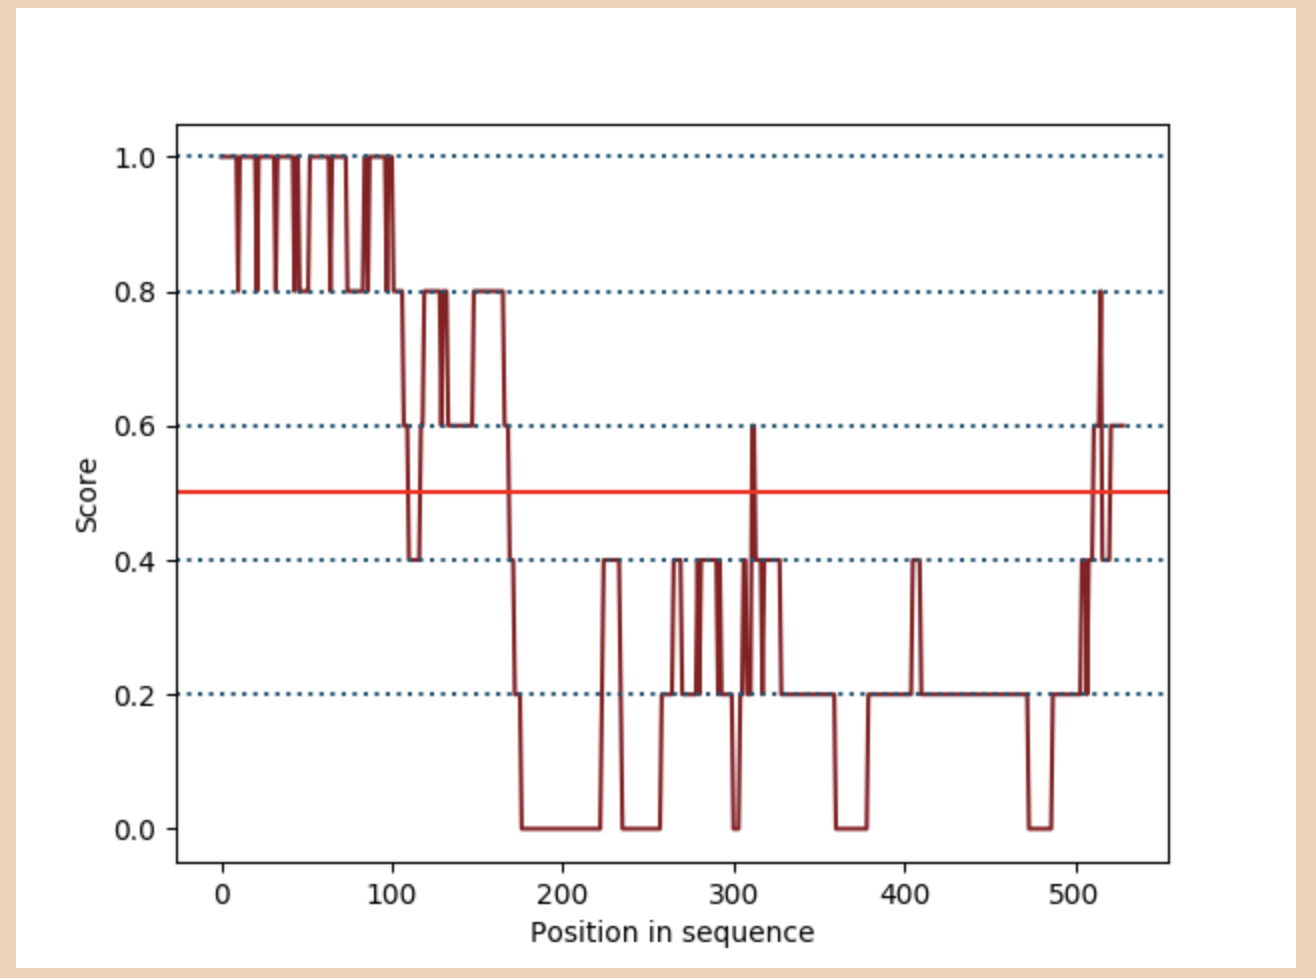
\includegraphics[width=0.5\textwidth]{Figures/App/sixth_screen.png}
    \caption{Prikaz dobijenih rezultata na grafiku}
    \label{fig:grafik}
\end{figure}

S obzirom da su analizirane i mere kvaliteta za metaprediktore za $k$ prediktora, njihov prikaz se vrši na samom dnu strane u vidu tabele prikazane na \ref{fig:detailed}. U tabeli su navedene mere i broj prediktora koji je korišćen. Napominje se još jednom da su mere kvaliteta vidljive u rezultatima samo ukoliko postoji $DisProt$ identifikator.
\begin{figure}[H]
	\centering
    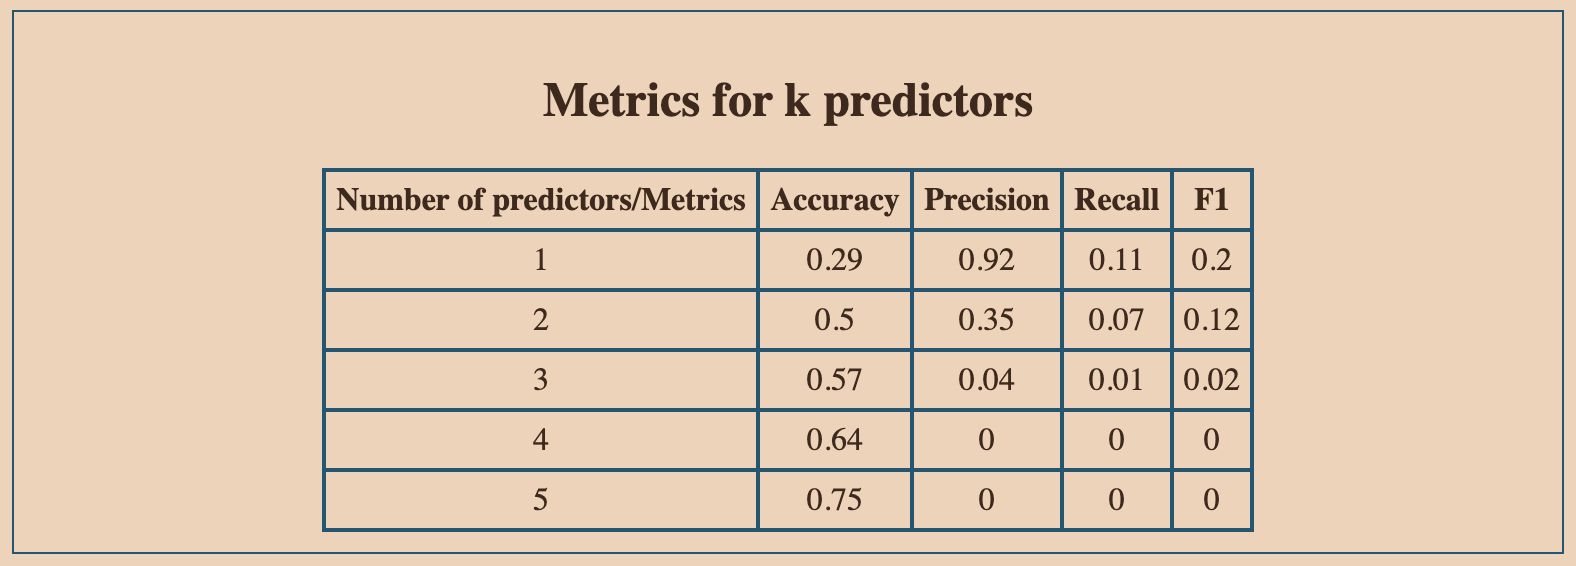
\includegraphics[width=0.7\textwidth]{Figures/App/detailed.png}
    \caption{Prikaz dobijenih rezultata u tabeli}
    \label{fig:detailed}
\end{figure}

Pored svega navedenog, u vrhu strane nalaze se dugmići koji se odnose na dodatne informacije, kao što su o projektu i uputstvo. Klikom na dugme $About$ dobijaju se detaljnije informacije o autoru, motivacija, cilj i korišćene mere, kao što se može videti na slici \ref{fig:about}, dok se detaljno uputstvo za korišćenje aplikacije nalazi na stranici instrukcije koja je prikazana na slici  \ref{fig:instr}.
\begin{figure}[H]
	\centering
    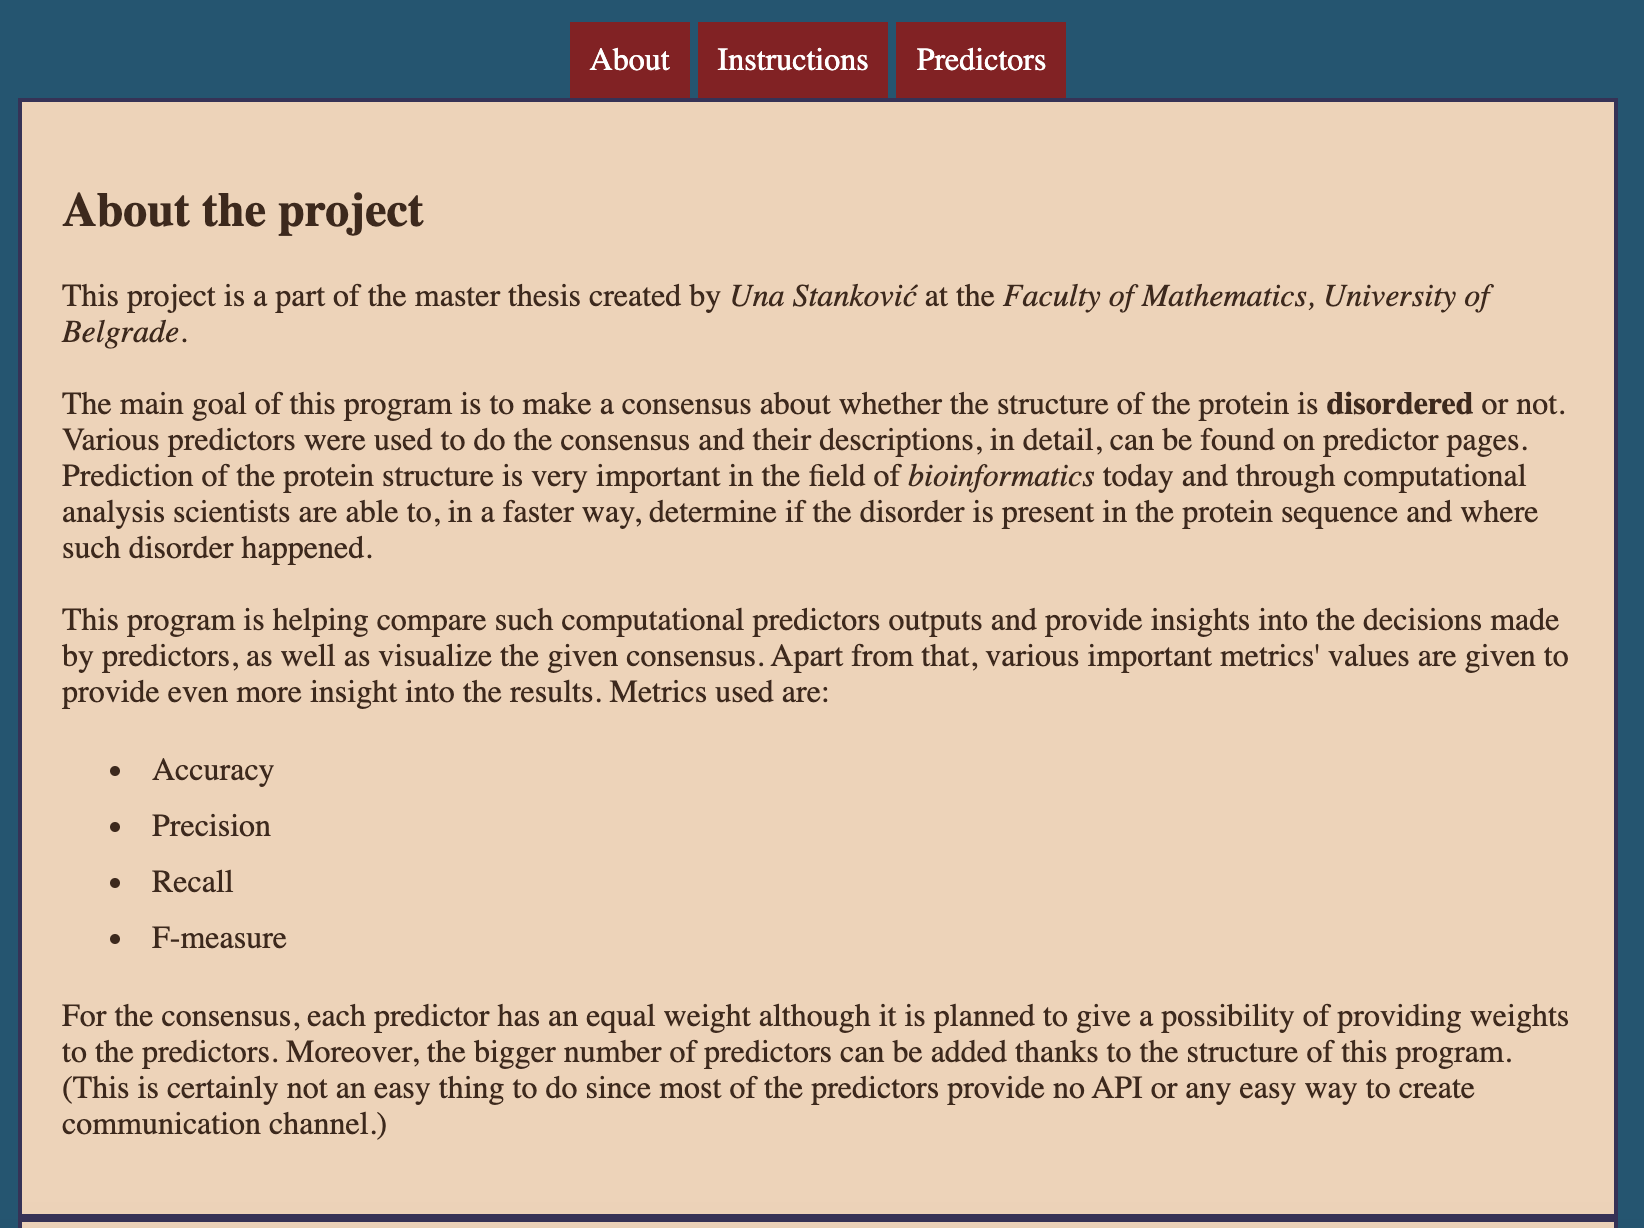
\includegraphics[width=0.7\textwidth]{Figures/App/about.png}
    \caption{Prikaz stranice koja se odnosi na dodatne informacije}
    \label{fig:about}
\end{figure}
\begin{figure}[H]
	\centering
    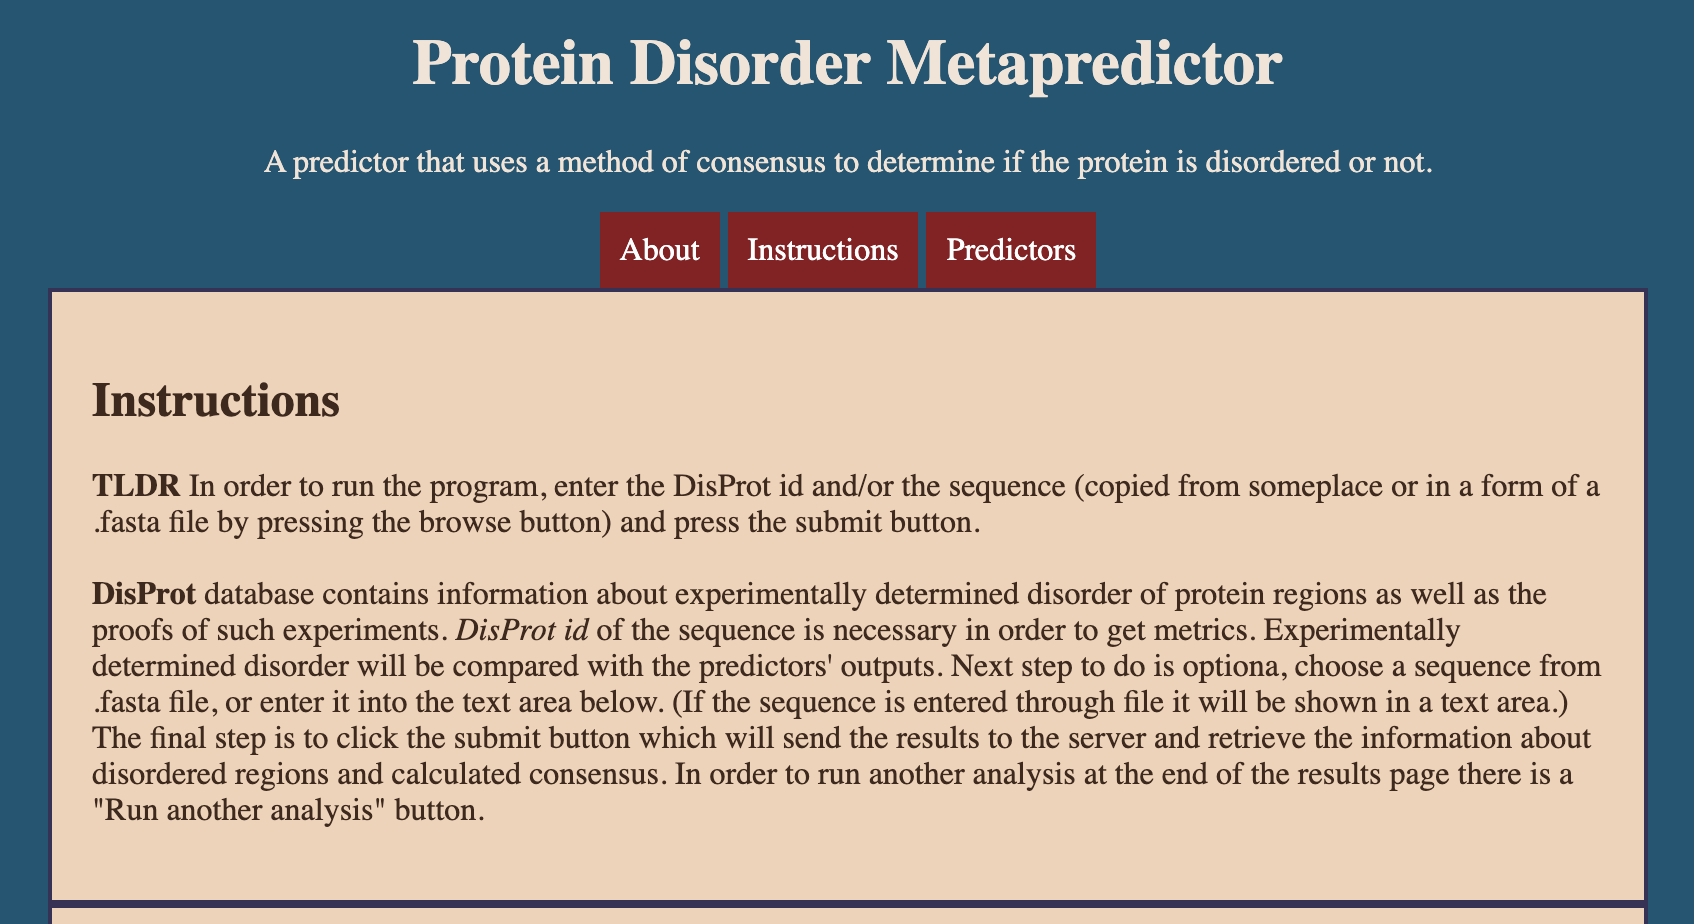
\includegraphics[width=0.7\textwidth]{Figures/App/instructions.png}
    \caption{Prikaz stranice sa uputstvom za korišćenje aplikacije}
    \label{fig:instr}
\end{figure}

\subsubsection{Drugi primer - zadavanje sekvence iz datoteke i prediktora}
Naredni primer predstavlja primer upotrebe zadavanjem sekvence iz datoteke i odabirom nekih od prediktora iz liste dostupnih. Sekvenca je preuzeta iz $UniProt$ baze i reč je o sekvenci sa $DisProt$ identifikatorom $DP00005$, ali on neće biti unesen.\\

Klikom na dugme $Browse$ bira se datoteka iz lokalnog direktorijuma. Odabir prediktora vrši se klikom na dugme za odabir pored imena prediktora, što se može videti na slici \ref{fig:DP51}. Odabrani prediktori su $IUPRED$ i $PONDR$.

\begin{figure}[H]
	\centering
    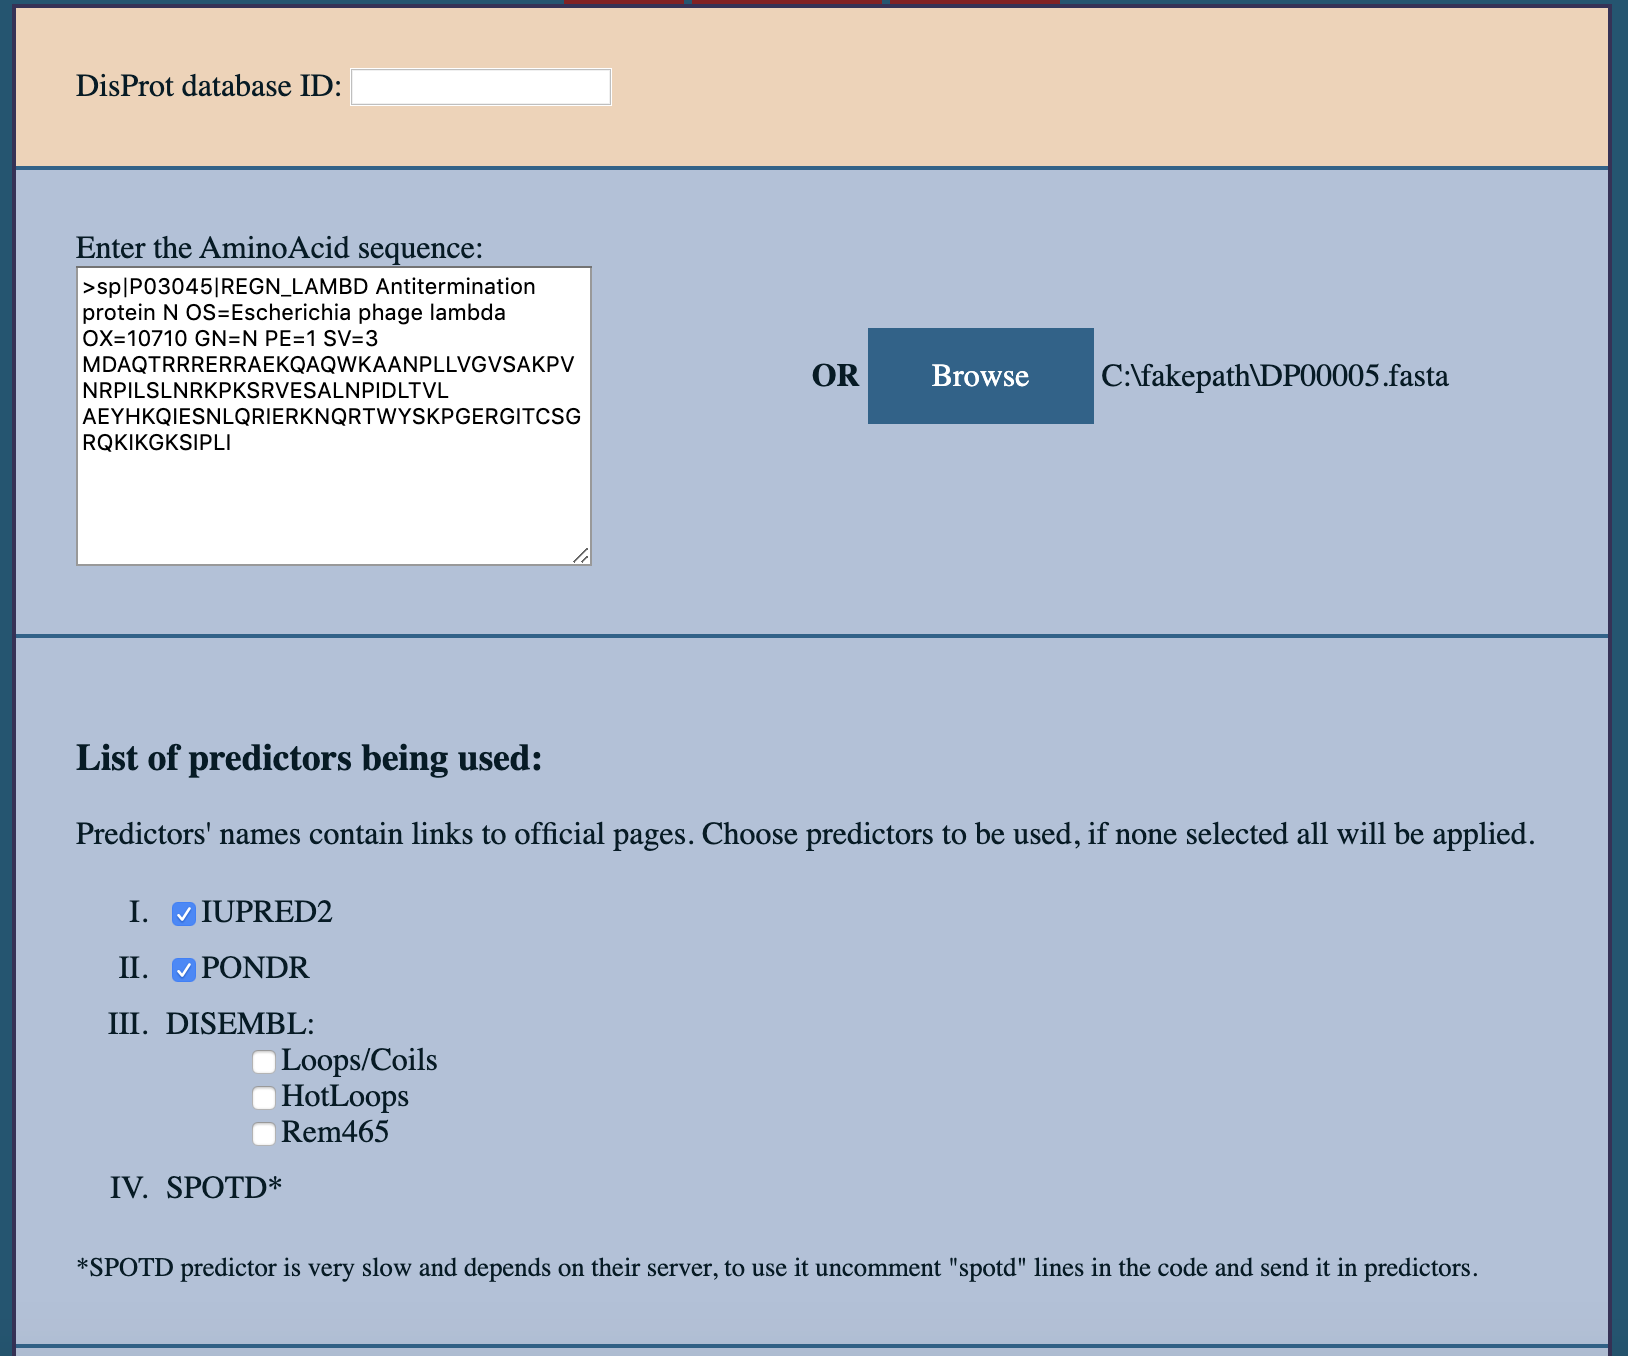
\includegraphics[width=0.7\textwidth]{Figures/App/DP00005/first_screen.png}
    \caption{Prikaz stranice sa unosom datoteke preko $Browse$ dugmeta i odabirom prediktora}
    \label{fig:DP51}
\end{figure}

Klikom na $Submit$ dugme podaci o odabranoj sekvenci i prediktorima šalju se na server, koji potom vraća odgovor. Odgovor ne sadrži mere kvaliteta, kao ni sekvencu u $DisProt$ bazi, zato što njen identifikator nije zadat. Na slikama \ref{fig:DP52} i \ref{fig:DP53} prikazan je celokupni odgovor servera.

\begin{figure}[H]
	\centering
    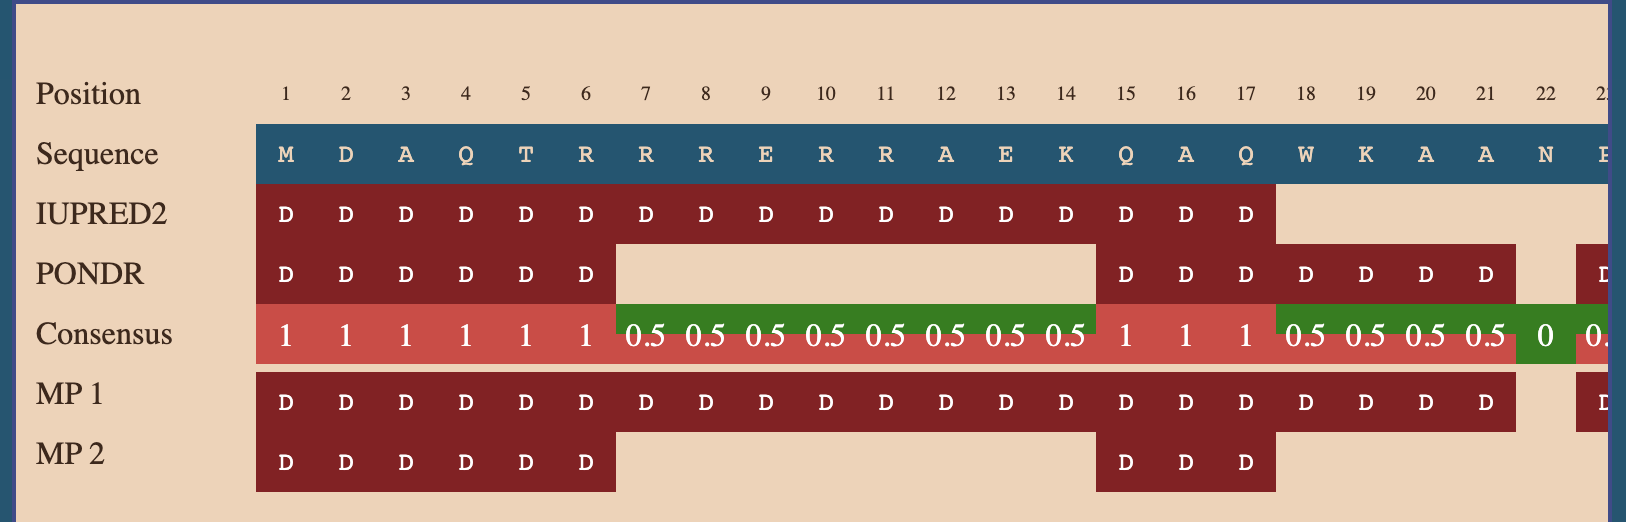
\includegraphics[width=0.7\textwidth]{Figures/App/DP00005/second_screen.png}
    \caption{Prikaz stranice sa rezultatima koje je vratio server}
    \label{fig:DP52}
\end{figure}

\begin{figure}[H]
	\centering
    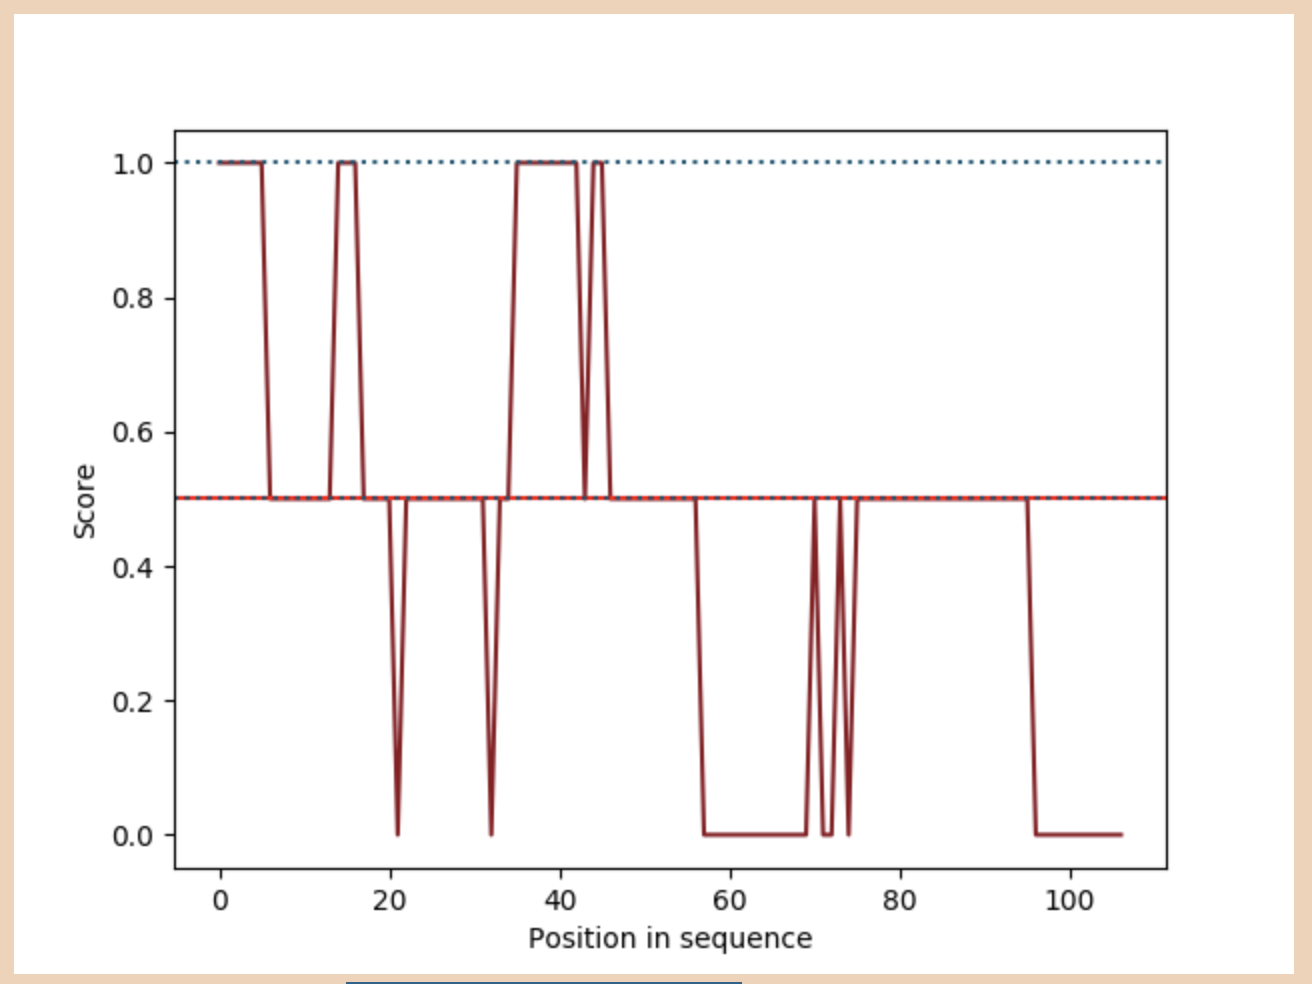
\includegraphics[width=0.5\textwidth]{Figures/App/DP00005/third_screen.png}
    \caption{Prikaz grafika sa rezultatima koje je vratio server}
    \label{fig:DP53}
\end{figure}

Odgovor od servera sadrži samo prediktore koji su zadati od strane korisnika, na osnovu kojih se računa prosečna vrednost skora prediktora. Na grafiku se iscrtavaju pragovi na osnovu broja prediktora. 

\section{Procena kvaliteta}
Kao što je ranije navedeno, funkcionalnosti ove aplikacije ogledaju se u uporednoj analizi izlaza više prediktora. Osim što se izlazi prediktora mogu uporediti vizuelnim putem, posmatranjem tabele ili grafika, dati su i rezultati nekoliko statističkih mera koje pružaju formalniji uvid u rezultate metaprediktora. 

\subsection{Merenje pouzdanosti metaprediktora}
%Kako bi se stekla jasnija slika stanja proteina koje su vratili prediktori neophodno je da osim vizuelnog prikaza postoji i formalno merilo kvaliteta metaprediktora.
 Za potrebe procene kvaliteta dobijenih rezultata predikcije korišćene su statističke mere:
\begin{itemize}
\item Preciznost (eng. \em{precision}), 
\item Odziv (eng.  \em{recall}), 
\item Tačnost (eng. \em{accuracy}) i 
\item F-mera (eng. \em{F-measure}). 
\end{itemize} 
%Ove mere su pogodne kako bi se utvrdilo koliko dobro metaprediktor predviđa u odnosu na eksperimentalno utvrđenu neuređenost. 
Procena kvaliteta predikcije vrši se u odnosu na informacije o eksperimentalno utvrđenim neuređenim regionima dobijenim iz $DisProt$ baze.\\

Pristup korišćen za prikaz vrednosti mera kvaliteta metaprediktora dobijenih poređenjem rezultata prosečne vrednosti skora svih prediktora sa pragom $0.5$ i eksperimentalno utvrđenih neuređenih regiona. Ovim pristupom, procenjuje se kvalitet rezultata kompletnog metaprediktora. U pojedinim situacijama, primećuje se da rezultati metaprediktora nisu uvek u skladu sa eksperimentalno utvrđenim rezultatima, već se u značajnoj meri razlikuju. Razlog ove pojave može se tražiti u nesavršenosti samih prediktora koji učestvuju u konsenzusu, kao i u potencijalno niskoj pokrivenosti rezultata eksperimenata nad određenim proteinima. \\
Za svaki prediktor su izračunate mere kvaliteta metaprediktora za vrednosti dobijene odnosom konsenzusa $k$ prediktora ($1\leq k \leq n, n=5$ ) i eksperimentalno utvrđenih neuređenih regiona.  Ovim pristupom merimo rezultate dobijene posmatranjem manjeg ili većeg broja prediktora i konsenzusa njihovih odluka. Vrednosti metrika koje se dobijaju ovim putem vrlo često se, posebno za $odziv$ i $F$-meru, svode na $0$ što je i razumljivo s obzirom na to da treba da se uklopi nekoliko faktora:
\begin{enumerate}
\item više od $k$ prediktora treba da utvrdi za neki region da je neuređen.
\item da bi taj region bio uzet u obzir, potrebno je da se rezultat prediktora poklopi sa rezultatima iz $DisProt$ baze.  
\end{enumerate}

U tabeli \ref{table:2} nalazi se prikaz metrika za sekvencu sa identifikatorom $DP00003$, dok se u tabelama \ref{table:5} i \ref{table:3}  nalaze se prikazi metrika za sekvence sa identifikatorima $DP00004$ i $DP00005$. Ove sekvence su odabrane kako bi se pokazala razlika u dobijenim metrikama u odnosu na to koliko aminokiselina 	je vraćeno iz baze kao neuređeno. $DP00003$ predstavlja jednu reprezentativnu sekvencu - ima i uređene i neuređene regione. Sa druge strane, sekvence $DP00004$ i $DP00005$ predstavljaju dve krajnosti. Naime, prva sekvenca je u potpunosti eksperimentalno uređena, dok je druga eksperimentalno u potpunosti neuređena. Nakon što program prikaže rezultate predikcije za sve tri sekvence može se videti da je broj mera sa ne-nula vrednostima značajno veći kod sekvence $DP00005$ što se može videti u tabeli \ref{table:3}. To se može objasniti time što je cela sekvenca $DP00005$ neuređena, čime se praktično posmatra samo izlaz iz metaprediktora. Sa druge strane, kod sekvence $DP00004$ prisutne su mere kvaliteta samo za prvu kolonu - tačnost, gde vrednosti značajno rastu kada se u analizu uključi više od dva prediktora. Vrednost za ostale mere su $0$.	

\begin{table}[H]
\centering
 \begin{tabular}{||c c c c c||} 
 \hline
 Broj prediktora/Metrika & Tačnost & Preciznost & Odziv & Fmera\\ [0.5ex] 
 \hline\hline
 1 & 0.29 & 0.92 & 0.11 & 0.2 \\ 
 \hline
 2 & 0.5 & 0.35 & 0.07 & 0.12 \\
 \hline
 3 & 0.64 & 0 & 0 & 0 \\
 \hline
 4 & 0.64 & 0 & 0 & 0\\
 \hline
 5 & 0.75 & 0 & 0 & 0\\ [1ex] 
 \hline
\end{tabular}
\caption{Prikaz mera kvaliteta metaprediktora za sekvencu DP00003}
\label{table:2}
\end{table}

\begin{table}[H]
\centering
 \begin{tabular}{||c c c c c||} 
 \hline
 Broj prediktora/Metrika & Tačnost & Preciznost & Odziv & Fmera\\ [0.5ex] 
 \hline\hline
 1 & 0.18 & 0 & 0 & 0 \\ 
 \hline
 2 & 0.45 & 0 & 0 & 0 \\
 \hline
 3 & 0.94 & 0 & 0 & 0 \\
 \hline
 4 & 0.94 & 0 & 0 & 0\\
 \hline
 5 & 0.99 & 0 & 0 & 0\\ [1ex] 
 \hline
\end{tabular}
\caption{Prikaz mera kvaliteta metaprediktora za sekvencu DP00004}
\label{table:5}
\end{table}

\begin{table}[H]
\centering
 \begin{tabular}{||c c c c c||} 
 \hline
 Broj prediktora/Metrika & Tačnost & Preciznost & Odziv & Fmera\\ [0.5ex] 
 \hline\hline
 1 & 0.89 & 0.89 & 1 & 0.94\\ 
 \hline
 2 & 0.83 & 0.83 & 1 & 0.91 \\
 \hline
 3 & 0.58 & 0.58 & 1 & 0.73 \\
 \hline
 4 & 0.12 & 0.12 & 1 & 0.22\\
 \hline
 5 & 0 & 0 & 0 & 0\\ [1ex] 
 \hline
\end{tabular}
\caption{Prikaz mera kvaliteta metaprediktora za sekvencu DP00005}
\label{table:3}
\end{table}
\newpage
\subsubsection{Procena mera kvaliteta nad DisProt bazom}
Kako bi se procenio kvalitet metaprediktora nad većem skupu sekvenci, metaprediktor je pušten nad svim sekvencama u $DisProt$ bazi. Preciznije, urađen je prosek procena mera kvaliteta dobijenih rezultata za svaki od metaprediktora koji koristi $k$ prediktora. Dobijeni rezultati predstavljeni su u tabeli \ref{table:finalni}.

\begin{table}[H]
\centering
 \begin{tabular}{||c c c c c||} 
 \hline
 Broj prediktora/Metrika & Tačnost & Preciznost & Odziv & Fmera\\ [0.5ex] 
 \hline\hline
 1 & 0.496 & 0.89 & 0.394 & 0.478 \\ 
 \hline
 2 & 0.647 & 0.678 & 0.452 & 0.477\\
 \hline
 3 & 0.697 & 0.265 & 0.491 & 0.299 \\
 \hline
 4 & 0.697 & 0.265 & 0.491 & 0.299\\
 \hline
 5 & 0.653 & 0.072 & 0.314 & 0.103\\ [1ex] 
 \hline
\end{tabular}
\caption{Prikaz mera kvaliteta metaprediktora za sve sekvence u $DisProt$ bazi}
\label{table:finalni}
\end{table}

    